\documentclass[]{article}
\usepackage{lmodern}
\usepackage{amssymb,amsmath}
\usepackage{ifxetex,ifluatex}
\usepackage{fixltx2e} % provides \textsubscript
\ifnum 0\ifxetex 1\fi\ifluatex 1\fi=0 % if pdftex
  \usepackage[T1]{fontenc}
  \usepackage[utf8]{inputenc}
\else % if luatex or xelatex
  \ifxetex
    \usepackage{mathspec}
  \else
    \usepackage{fontspec}
  \fi
  \defaultfontfeatures{Ligatures=TeX,Scale=MatchLowercase}
\fi
% use upquote if available, for straight quotes in verbatim environments
\IfFileExists{upquote.sty}{\usepackage{upquote}}{}
% use microtype if available
\IfFileExists{microtype.sty}{%
\usepackage{microtype}
\UseMicrotypeSet[protrusion]{basicmath} % disable protrusion for tt fonts
}{}
\usepackage[margin=1in]{geometry}
\usepackage{hyperref}
\hypersetup{unicode=true,
            pdftitle={Standardization \& Balancing for Food Balance Sheet Calculation},
            pdfauthor={Cristina Muschitiello Food and Agriculture Organization of the United Nations},
            pdfborder={0 0 0},
            breaklinks=true}
\urlstyle{same}  % don't use monospace font for urls
\usepackage{graphicx,grffile}
\makeatletter
\def\maxwidth{\ifdim\Gin@nat@width>\linewidth\linewidth\else\Gin@nat@width\fi}
\def\maxheight{\ifdim\Gin@nat@height>\textheight\textheight\else\Gin@nat@height\fi}
\makeatother
% Scale images if necessary, so that they will not overflow the page
% margins by default, and it is still possible to overwrite the defaults
% using explicit options in \includegraphics[width, height, ...]{}
\setkeys{Gin}{width=\maxwidth,height=\maxheight,keepaspectratio}
\IfFileExists{parskip.sty}{%
\usepackage{parskip}
}{% else
\setlength{\parindent}{0pt}
\setlength{\parskip}{6pt plus 2pt minus 1pt}
}
\setlength{\emergencystretch}{3em}  % prevent overfull lines
\providecommand{\tightlist}{%
  \setlength{\itemsep}{0pt}\setlength{\parskip}{0pt}}
\setcounter{secnumdepth}{5}
% Redefines (sub)paragraphs to behave more like sections
\ifx\paragraph\undefined\else
\let\oldparagraph\paragraph
\renewcommand{\paragraph}[1]{\oldparagraph{#1}\mbox{}}
\fi
\ifx\subparagraph\undefined\else
\let\oldsubparagraph\subparagraph
\renewcommand{\subparagraph}[1]{\oldsubparagraph{#1}\mbox{}}
\fi

%%% Use protect on footnotes to avoid problems with footnotes in titles
\let\rmarkdownfootnote\footnote%
\def\footnote{\protect\rmarkdownfootnote}

%%% Change title format to be more compact
\usepackage{titling}

% Create subtitle command for use in maketitle
\newcommand{\subtitle}[1]{
  \posttitle{
    \begin{center}\large#1\end{center}
    }
}

\setlength{\droptitle}{-2em}

  \title{Standardization \& Balancing\\
for Food Balance Sheet Calculation}
    \pretitle{\vspace{\droptitle}\centering\huge}
  \posttitle{\par}
    \author{Cristina Muschitiello\\
Food and Agriculture Organization of the United Nations}
    \preauthor{\centering\large\emph}
  \postauthor{\par}
      \predate{\centering\large\emph}
  \postdate{\par}
    \date{8 August 2018}

\usepackage{lscape}
\usepackage{booktabs}
\usepackage{longtable}
\usepackage{array}
\usepackage{multirow}
\usepackage[table]{xcolor}
\usepackage{wrapfig}
\usepackage{float}
\usepackage{colortbl}
\usepackage{pdflscape}
\usepackage{tabu}
\usepackage{threeparttable}
\usepackage{threeparttablex}
\usepackage[normalem]{ulem}
\usepackage{makecell}

\usepackage{draftwatermark}
\usepackage{makeidx}
\makeindex
\usepackage{float}
\floatplacement{figure}{H}
\usepackage{amsmath}
\usepackage{amssymb}
\usepackage{amsthm}
\usepackage{mathtools}
\usepackage{caption}

\begin{document}
\maketitle
\begin{abstract}
This vignette provides a description of the Standardization and
Balancing Procedure: This represents the process of aggregating and
balancing all the accounts of individual products to their primary
equivalents. Other documents will cover the overall Food Balance Sheet
workflow and some, more detailed, technical aspect.
\end{abstract}

{
\setcounter{tocdepth}{4}
\tableofcontents
}
\newpage

\listoftables

\listoffigures

\newpage

\subsection*{Disclaimer}\label{disclaimer}
\addcontentsline{toc}{subsection}{Disclaimer}

This Working Paper should not be reported as representing the official
view of the FAO. The views expressed in this Working Paper are those of
the author and do not necessarily represent those of the FAO or FAO
policy. Working Papers describe research in progress by the authors and
are published to elicit comments and to further discussion.

This paper is dynamically generated on \today{} and is subject to
changes and updates.

\section*{The Food Balance Sheet
Framework}\label{the-food-balance-sheet-framework}
\addcontentsline{toc}{section}{The Food Balance Sheet Framework}

\subsection*{Definitions}\label{definitions}
\addcontentsline{toc}{subsection}{Definitions}

A food balance sheet can be defined as an aggregated and analytic data
set that ``presents a comprehensive picture of the pattern of a
country's food supply during a specified reference period.''\footnote{For
  this definition and a more extended description of the motivation
  behind the development of FBS, see FAO, 2001, \emph{Food Balance
  Sheets: A Handbook}, available at:
  \url{http://www.fao.org/docrep/003/X9892E/X9892E00.HTM}. Accessed on
  19 January 2017.} FBS are presented as products accounts, where the
quantities allocated to all the sources of total supply must be equal to
the quantities allocated to all the sources of utilization. This balance
is compiled for every food item consumed within a country at primary
commodity equivalent basis, and all of the primary commodity equivalent
balances are then combined into a single overall FBS. FBSs are, then,
expressed in terms of per capita supply for each food item by dividing
by the country's population, with the per capita supplies being
expressed both in terms of quantity and, through the application of food
conversion factors, in terms of caloric value, protein, and fat content.
These per capita estimates of caloric value for individual food products
are then summed to obtain the total daily per capita Dietary Energy
Supply (DES) of a country.

While FBS are typically only published at the primary commodity
equivalent level to facilitate interpretation, they are created for all
the commodities, accordingly to the \emph{Central Product
Classification} (\textbf{\emph{CPC}}) System\footnote{The CPC represents
  a comprehensive classification of products into a system of categories
  that are both exhaustive and mutually exclusive. It is based on a set
  of internationally agreed concepts, definitions, principles and
  classification rules. The custodian of this classification is the
  UNSD. For more information, see the
  \href{http://gsars.org/wp-content/uploads/2015/12/Guidelines-for-Int-Classifications-on-Agricultural-Statistics-web.pdf}{\emph{Guidelines
  on International Classifications for Agricultural Statistics}} and the
  \href{https://unstats.un.org/unsd/cr/downloads/CPCv2.1_complete\%28PDF\%29_English.pdf}{\emph{UNSD
  official document on CPC Version 2.1}}}. Indeed, a balance for wheat
alone would in most cases include little or no food use, because wheat
is commonly processed into flour before it is consumed by humans, and
flour is then used to produce various other derived products such as
bread, pastries and pasta. Because there is both supply and demand both
for the primary commodity and the derived commodities, individual
accounts are kept for all of products. Individual accounts for
commodities are called \emph{Supply-Utilization Accounts}
(\textbf{\emph{SUA}}) and the process of obtaining FBS starting from
SUAs is the \textbf{\emph{Standardization \& Balancing}} process.

\subsection*{The Balancing equation and its
variables}\label{the-balancing-equation-and-its-variables}
\addcontentsline{toc}{subsection}{The Balancing equation and its
variables}

At the most basic level, Food Balance Sheets are, like all commodity
balances, simple identities. In these identities, the sum of all supply
variables is equal to the sum of all demand variables; the two most
common identities set domestic supply equal to domestic demand (first
equation) or total supply equal to total demand (second equation).

\begin{equation}
\label{eq:balance1}
P_{ijt} + I_{ijt} - X_{ijt} - \Delta St_{ijt} = FP_{ijt} + Fo_{ijt} + Fe_{ijt} + Lo_{ijt} + Se_{ijt} + IU_{ijt} + T_{ijt}  + ROU_{ijt}
\end{equation}\begin{equation}
\label{eq:balance2}
P_{ijt} + I_{ijt} - \Delta St_{ijt} = X_{ijt} + FP_{ijt} + Fo_{ijt} + Fe_{ijt} + Lo_{ijt} + Se_{ijt} + IU_{ijt} + T_{ijt} + ROU_{ijt}
\end{equation}

where the \(i\) index runs over all countries, the \(j\) index over all
commodities, and \(t\) over years and where, dropping indices for
brevity:

\begin{itemize}
\tightlist
\item
  \(P\)=Production
\item
  \(I\)=Imports
\item
  \(X\)=Exports
\item
  \(S\)=Stock level
\item
  \(\Delta St_{t}\) = Stock Variation = \(St_{t} - St_{t-1}\)
\item
  \(FP_{ijt}\) = Food Processing
\item
  \(Fo\)=Food availability
\item
  \(Fe\)=Feed
\item
  \(Lo\)=Losses
\item
  \(Se\)=Seed
\item
  \(IU\)=industrial use
\item
  \(T\)=Tourist consumption
\item
  \(ROU\)=Residual Other Use
\item
  \(TS = Total supply = P_{ijt} + I_{ijt} - \Delta St_{ijt}\)
\end{itemize}

All variables are expressed in the same measurement unit:
\textbf{\emph{metric tonnes}}. At international level, the primary data
source that FAO uses to compile the the Supply Utilization Accounts/Food
Balance Sheets are the data as collected through the annual
\emph{Agriculture Production Questionnaires}. Unfortunately, measured
values are mostly limited to variables on the supply side (production,
imports and exports), while, on the demand side, most values are imputed
data\footnote{For more details on FBS variables please see the latest
  version of the \emph{Resource Book}, the documentation on \emph{Food
  Balance Sheet workflow in the Statistical Working System} to be found
  on
  \href{https://github.com/SWS-Methodology/faoswsStandardization/tree/master/documentation}{\emph{GitHub}}
  and \href{https://sdlc.fao.org/bitbucket/projects}{\emph{Bitbucket}}
  and specific documentation available about imputation of all variables}:

\section*{Commodity Tree}\label{commodity-tree}
\addcontentsline{toc}{section}{Commodity Tree}

The process of combining commodity balances for creating Food Balance
Sheets is based on a structured and clear set of relationships between
commodity given by the \emph{Commodity tree}. The majority of the
commodities are produced from one (or more) commodity (/ies), called
\emph{parent} commodity(/ies), and/or are themselves parent of one (or
more) \emph{child} (\emph{children}) commodity (/ies). These structure
creates an intense and articulated network of relationships at different
levels: primary commodities, like crops, are \emph{parent} commodities
and, also, \emph{zero-level} commodities from which \emph{children}
commodities of \emph{level-1} are produced, which are in turn, used to
produce other commodities of a gradually \emph{``lower''} level. In
commodity trees, the bigger the level number, the lower the processing
level. There are as many commodity trees as the number of process chains
in a country. Fundamental characteristics of commodity trees
are\footnote{For a more detailed description of commodity trees, please
  see the specific documentation. The reference document, at the moment
  is the \emph{tecnical conversion factor} document available in the
  documentation folder on
  \href{https://github.com/SWS-Methodology/faoswsStandardization/tree/master/documentation}{\emph{GitHub}}}:

\begin{enumerate}
\def\labelenumi{\arabic{enumi}.}
\tightlist
\item
  Each commodity tree is represented as a flowchart of the kind
  presented in Figure \ref{fig:f2} where:

  \begin{itemize}
  \tightlist
  \item
    \textbf{\emph{nodes}} represent commodities,
  \item
    \textbf{\emph{edges}} represent production processes ,
  \item
    \textbf{\emph{joints}} indicate where a single production process
    creates more that one commodity. These commodities are, then, called
    \emph{by-products} or \emph{co-products}.
  \end{itemize}
\end{enumerate}

\begin{figure}[H]

{\centering 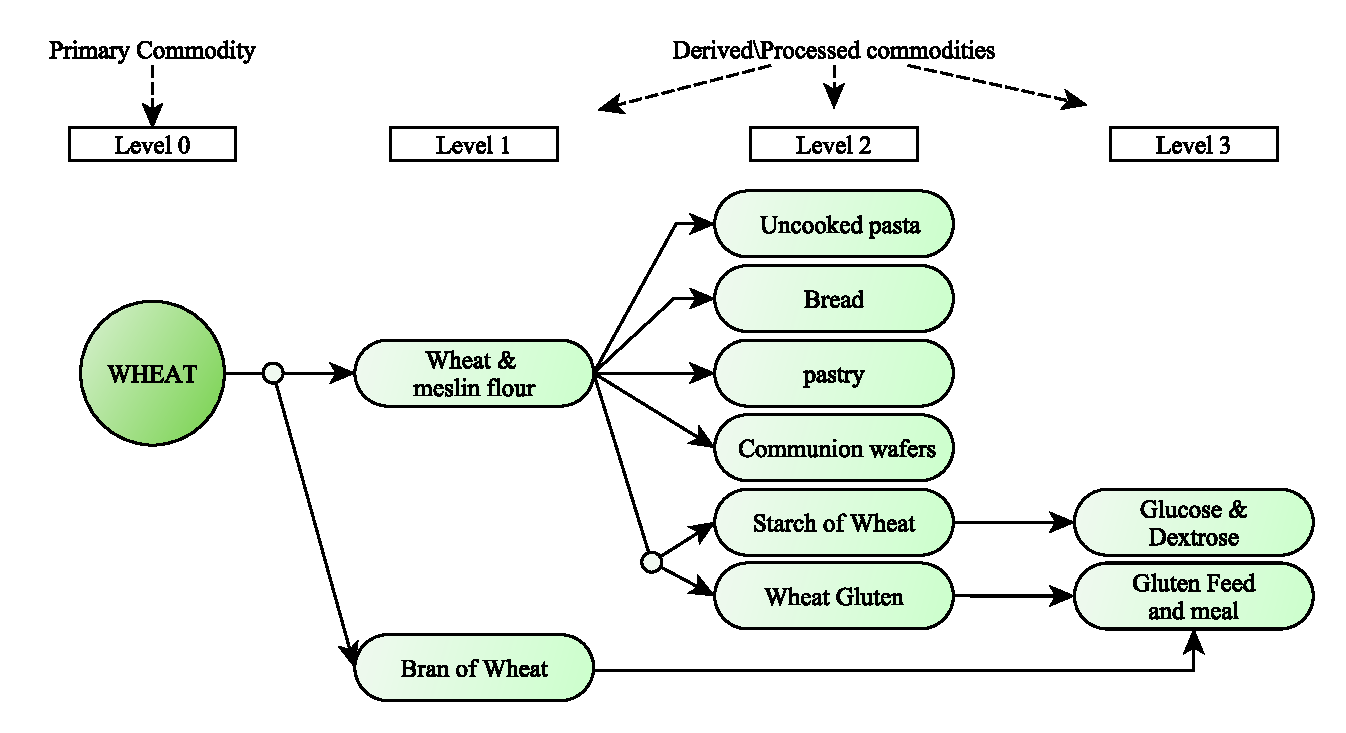
\includegraphics{images/StandBal/02_WheatTree} 

}

\caption{\label{fig:f2}Commodity Tree for Wheat in China mainland 2014}\label{fig:f2}
\end{figure}

\begin{enumerate}
\def\labelenumi{\arabic{enumi}.}
\setcounter{enumi}{1}
\item
  Not all the countries have the same production processes: countries
  have different technologies and primary products availability.
  Therefore, the commodity trees are not the same across countries.
\item
  if a production process is active in a country, this is expressed
  through the existence of a conversion factor called
  \textbf{\emph{extraction Rate}}. An Extraction rate (\(eR\))
  represents how much amount of the child commodity is produced from 1
  unit of parent commodity. It is expressed as a ratio of the processed
  product obtained from the processing of the parent/originating
  product.
\item
  Some child commodities can be produced starting from more that one
  parent commodity. A second conversion factor exists representing the
  amount of a child commodity that is produced from each parent
  commodity. This conversion factor is called \textbf{\emph{Share}}.
  Shares represent the amount of the child commodity that is produced
  from the specified parent and are expressed as a ratio. Shares are
  generically defined as:
\end{enumerate}

\begin{quote}
\begin{equation}
\label{eq:sharesGen}
s_{cp} = \frac{availability_{p(c)}}{\sum \limits_{p=1}^A{availability_{p(c)}}}
\end{equation}
\end{quote}

\begin{quote}
where \(availability_{p(c)}\) is the availability of each parent \(p\)
of child \(c\) expressed in terms of \(c\) (in \emph{child equivalent}).
\end{quote}

Commodity trees are presented in tables like Table 1, which represents
the same example of Figure \ref{fig:f2}. In the table each production
process is represented in a separate row.

\begin{table}

\caption{\label{tab:t15}Commodity Tree - China/Wheat/2014 example}
\centering
\begin{tabular}[t]{r|l|l|l|l|l}
\hline
Country & Year & ParentName & ChildName & eR & share\\
\hline
China, Mainland & 2014 & Wheat & Wheat and meslin flo & 0.78 & 1.00\\
\hline
China, Mainland & 2014 & Wheat & Bran of Wheat & 0.22 & 1.00\\
\hline
China, Mainland & 2014 & Wheat and meslin flo & Uncooked pasta, not & 1.00 & 1.00\\
\hline
China, Mainland & 2014 & Wheat and meslin flo & bread & 1.00 & 1.00\\
\hline
China, Mainland & 2014 & Wheat and meslin flo & pastry & 1.00 & 1.00\\
\hline
China, Mainland & 2014 & Wheat and meslin flo & Starch of Wheat & 0.75 & 1.00\\
\hline
China, Mainland & 2014 & Wheat and meslin flo & Wheat Gluten & 0.08 & 1.00\\
\hline
China, Mainland & 2014 & Wheat and meslin flo & Communion wafers, em & 1.00 & 1.00\\
\hline
China, Mainland & 2014 & Starch of Wheat & Other Fructose and S & 1.00 & 1.00\\
\hline
China, Mainland & 2014 & Wheat Gluten & Gluten Feed and Meal & 1.00 & 0.33\\
\hline
China, Mainland & 2014 & Bran of Maize & Gluten Feed and Meal & 1.00 & 0.67\\
\hline
\end{tabular}
\end{table}

There are some concepts linked to the \emph{Commodity tree} framework:

\begin{itemize}
\tightlist
\item
  \textbf{\emph{Proxy-Primary}} commodities. These are a set of
  commodities that are children of other commodities but, because they
  are important in representing the food availability of a country, are
  not aggregated to their primary commodities, but are kept separated.
  These commodities are \emph{cut} from the tree of the primary
  commodity/ies and, if they can be processed in other products, have
  their own commodity tree. The name \emph{proxy-primary} is assigned
  because they are considered as primary-commodities in the
  \emph{Standardization \& Balancing} process.
\item
  \textbf{\emph{No-Tree}} commodities. These are \emph{zero-level}
  commodities. They are either primary commodities that are never
  processed (as lettuce) or commodities that are not processed in a
  specific country/commodity combination. As they are not involved in
  any production process, there is no tree associated to them. Notice
  that, even a commodity that is included in the commodity tree of one
  Country, might be a No-tree commodity for another country or another
  year. This happens if no production processes have been activated for
  that specific Country or year.
\end{itemize}

\section*{Standardization and
Balancing}\label{standardization-and-balancing}
\addcontentsline{toc}{section}{Standardization and Balancing}

The \emph{Standardiation \& Balancing} process is presented in Figure
\ref{fig:f9}. It involves 5 main steps and requires a some auxiliary
information table.

The 5 steps are:

\begin{enumerate}
\def\labelenumi{\arabic{enumi}.}
\tightlist
\item
  Data Pull,
\item
  Sua Filling,
\item
  Standardization,
\item
  Balancing,
\item
  FBS aggregation.
\end{enumerate}

The additional information's tables are:

\begin{itemize}
\tightlist
\item
  \emph{Utilization Table},
\item
  \emph{Zero-Weight} table,
\item
  \emph{cut} table,
\item
  \emph{Fbs Tree}.
\end{itemize}

\begin{figure}[H]

{\centering 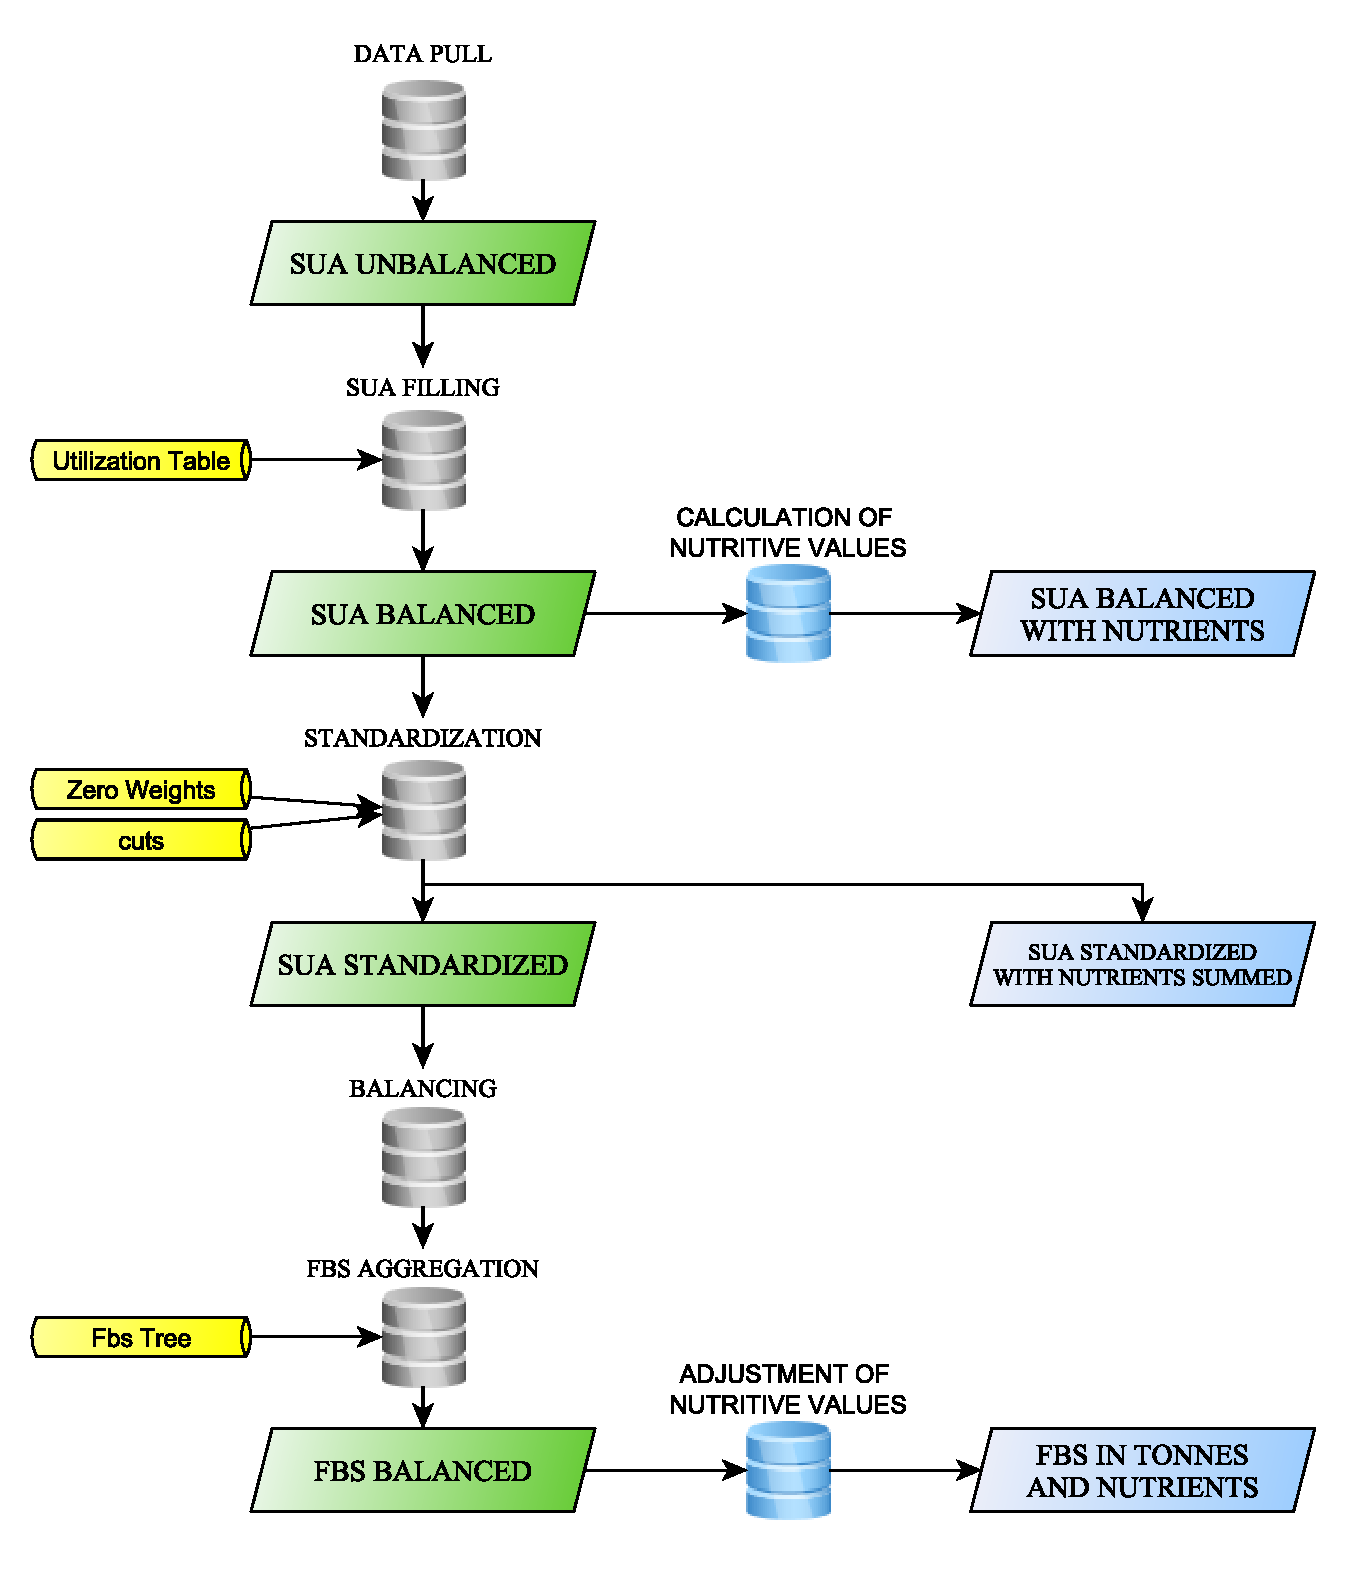
\includegraphics[width=0.8\linewidth]{images/StandBal/09_overall} 

}

\caption{\label{fig:f9}Standardization and Balancing Overall Workflow}\label{fig:f9}
\end{figure}

\section{Data Pull}\label{data-pull}

The process of creating FBSs starts by considering the initial commodity
balance for each CPC commodity, either primary and derived. In the
balance the different variables of the equation (as listed and briefly
described in the previous section) are filled with figures as available
from official or other sources and from imputation and estimation
methods, when applied. In other words, the process starts by pulling
figures inside a so-called \emph{Sua Unbalanced}.

In this initial account, food processing and ROU figures are not
available (because they, by default, will be measured during the
process), whereas the figures for all other variables have been already
collected, imputed and estimated through a specific \emph{module}
(Figure \ref{fig:f1}).

A \textbf{\emph{module}}, in the FBS Framework, is an R-script, written
by an R-developer, for the execution of a set of operations (either data
import, manipulation, imputation or estimation) required for compiling
the time series of one variable. There is at least one module (there
might be more) for each variable of the FBS. Each module produces
figures that are collected in a dataset inside the
\textbf{\emph{Statistical Working System (SWS)}}\footnote{SWS is an
  internal Working System providing a platform for statisticians and
  statistical clerks to collect, collate, validate and correct data.
  Moreover, the platform supports the possibility of performing
  imputations of data based on statisticians' knowledge and development.}.Output
data of a module may become input data of another module, this
circumstance creating a precise sequence for the execution of a complete
FBS. In the present document, we are analyzing the workflow of the
Standardization process as starts after all the modules have run and
have produced reliable data or each variable. The detailed description
of the workflow for the execution of all the modules of the FBS is given
in a separate document.\footnote{{[}report the document when it will be
  available{]}}.

\begin{figure}[htbp]
\centering
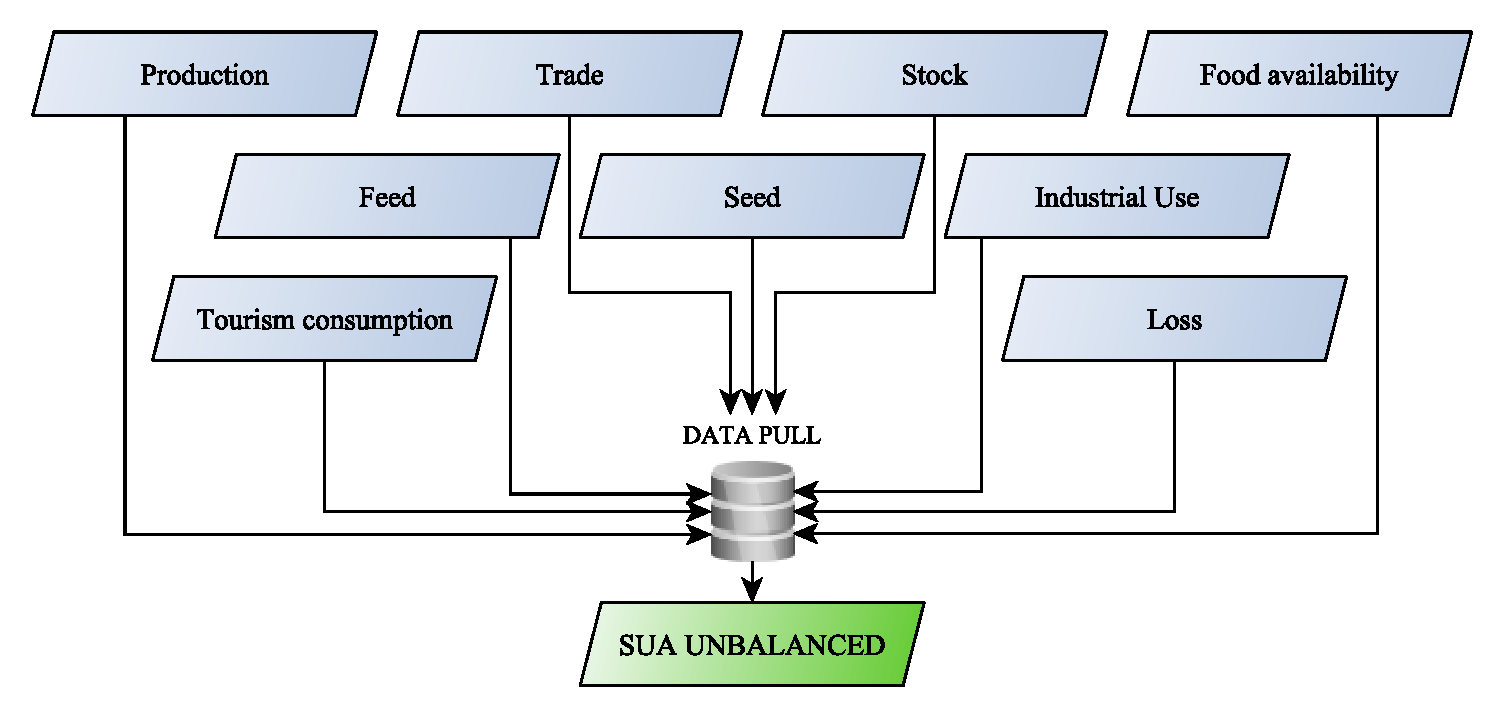
\includegraphics{images/StandBal/01_pulldata.pdf}
\caption{\label{fig:f1}Data Pull from datasets containing data for each
separate variable}
\end{figure}

\subsection*{The Initial Sua
Unbalanced}\label{the-initial-sua-unbalanced}
\addcontentsline{toc}{subsection}{The Initial Sua Unbalanced}

After pulling all data, the process of compiling Food Balance Sheets is
a non-complete supply-utilization account. The non-completeness of the
SUAs is due to different reasons: first, as already said, some variables
are not collected, nor estimated before the process begins. Second,
there is the model for industrial use that does not impute or estimate
data, but just collects data from different sources \footnote{this
  opening the strong possibility not to have values where they are
  supposed to exist and, also, not guaranteeing consistency of data over
  time}. Third, modules might, sometimes, fail in the imputation,
because of the strong complexity and structural diversity of the input
data.

\begin{landscape}\begin{table}

\caption{\label{tab:t1}Unbalanced Sua table - China/Wheat/2014 example}
\centering
\resizebox{\linewidth}{!}{
\fontsize{18}{20}\selectfont
\begin{tabular}[t]{>{\raggedleft\arraybackslash}p{12em}|>{\raggedright\arraybackslash}p{6em}|>{\raggedright\arraybackslash}p{6em}|>{\raggedright\arraybackslash}p{6em}|>{\raggedright\arraybackslash}p{6em}|>{\raggedright\arraybackslash}p{6em}|>{\raggedright\arraybackslash}p{6em}|>{\raggedright\arraybackslash}p{6em}|>{\raggedright\arraybackslash}p{6em}|>{\raggedright\arraybackslash}p{6em}|>{\raggedright\arraybackslash}p{6em}|>{\raggedright\arraybackslash}p{6em}|>{\raggedright\arraybackslash}p{6em}}
\hline
\multicolumn{1}{r}{\textbf{itemName}} & \multicolumn{1}{c}{\textbf{P}} & \multicolumn{1}{c}{\textbf{I}} & \multicolumn{1}{c}{\textbf{X}} & \multicolumn{1}{c}{\textbf{DSt}} & \multicolumn{1}{c}{\textbf{Fo}} & \multicolumn{1}{c}{\textbf{FP}} & \multicolumn{1}{c}{\textbf{Fe}} & \multicolumn{1}{c}{\textbf{Se}} & \multicolumn{1}{c}{\textbf{T}} & \multicolumn{1}{c}{\textbf{IU}} & \multicolumn{1}{c}{\textbf{L}} & \multicolumn{1}{c}{\textbf{ROU}}\\
\hline
\em{Wheat} & \em{126,208,400} & \em{2,971,249} & \em{957} & \em{1,120,565} & \em{} & \em{-} & \em{29,181,617} & \em{4,277,567} & \em{} & \em{2,985,279} & \em{2,713,000} & \em{-}\\
\hline
Wheat and meslin flo & 70,500,000 & 33,055 & 188,674 &  & 67,300,000 & - &  &  & -17,345 &  &  & -\\
\hline
Mixes and doughs for &  & 6,497 & 38,072 &  & 0 & - & 0 &  & 0 &  &  & -\\
\hline
Other Fructose and S & 126,277 & 3,659 & 162,324 &  & 0 & - &  &  & 0 &  &  & -\\
\hline
Starch of Wheat & 239,816 & 11,035 & 40,311 &  &  & - & 172,196 &  &  & 7,919 &  & -\\
\hline
Wheat Gluten & 25,580 & 877 & 117,373 &  &  & - & 0 &  &  &  &  & -\\
\hline
Communion wafers & 13,263 & 8,796 & 5,822 &  & 16,241 & - &  &  & -4 &  &  & -\\
\hline
Uncooked pasta & 1,415,692 & 12,520 & 22,550 &  & 1,405,661 & - &  &  & -362 &  &  & -\\
\hline
Food Preparations of &  & 69,686 & 21,977 &  & 47,709 & - &  &  & -12 &  &  & -\\
\hline
Bran of Wheat & 21,414,279 & 156,359 & 2,200 &  & 16,500,000 & - & 4,827,244 &  & -4,252 &  &  & -\\
\hline
Gluten Feed and Meal & 793,740 & 160,231 & 529,333 &  &  & - &  &  &  &  &  & -\\
\hline
bread & 15,485 & 2,897 & 4,210 &  & 14,175 & - &  &  & -3 &  &  & -\\
\hline
pastry & 193,950 & 89,593 & 117,630 &  & 165,914 & - &  &  & -43 &  &  & -\\
\hline
\multicolumn{13}{l}{\textsuperscript{a} P=Production, I=Import, X=Export, DSt=Delta Stock, Fo=Food Availability, FP=FoodProcessing, Fe=Feed, Se=Seed, T=Tourism Consumption, IU=IndustrialUse, L=Loss, ROU=Residual and other uses}\\
\end{tabular}}
\end{table}
\end{landscape}

Supply utilization accounts are typically organized into tables where
the SUA for the primary commodity is at the top, and the SUAs for all of
the products derived from that commodity follow (Table 2). Commodities
in the SUA table are in a parent-child relationship representing a real
commodity process. In the example of Table 2 the relationship between
commodities is the following:

\begin{itemize}
\tightlist
\item
  Maize is processed in flour, Bran and Breakfast Cereals,
\item
  Flour of maize is processed into Starch and Gluten, Wafers, pastry,
  bread and pasta
\item
  Starch is processed into Glucose and Dextrose,
\item
  Gluten and Bran are processed into some feed and meal,
\end{itemize}

All these relationships represent the \emph{Commodity tree} of wheat in
China in 2014. In particular, our example represents the commodity tree
of Wheat in China in 2014 and is displayed, in its graphical form, in
Figure \ref{fig:f2}.

A \emph{SUA} also contains other commodities, when existing, that are
associated to the primary commodity inside an FBS item. In our example,
the \emph{SUA} table includes the commodity \emph{Mixes and dough for
the preparation of baker's wares} because it is included in the FBS
commodity \emph{WHEAT \& PRODUCTS}. That commodity is in the \emph{SUA}
of Wheat even if is not processed from wheat directly and is not
processed in any commodity. It is a No-tree commodity.

\section{\texorpdfstring{The \emph{Sua
Filling}}{The Sua Filling}}\label{the-sua-filling}

\subsection*{Main rules and the
rationale}\label{main-rules-and-the-rationale}
\addcontentsline{toc}{subsection}{Main rules and the rationale}

The Standardization, i.e.~the conversion of the variables of any child
commodity in primary-equivalent commodity, requires all variables of the
SUAs to be filled (except for ROU, which is a residual variable and is
imputed at the very last step of the process). ``All variables'' here
means ``all variables that are supposed to be filled''. Indeed, not all
variables have to exist for all commodities. Consider maize as an
example: if there is no figure of \emph{food availability} for maize,
that does not mean that there is a missing figure because maize is
rarely used for human consumption directly. However, in some country
people do eat raw maize and, therefore, for those countries, a food
figure is expected and, if missing, that has to be taken into account.

A simplified workflow of \emph{Sua Filling} is reported in Figure
\ref{fig:f3}.

\begin{figure}[H]

{\centering 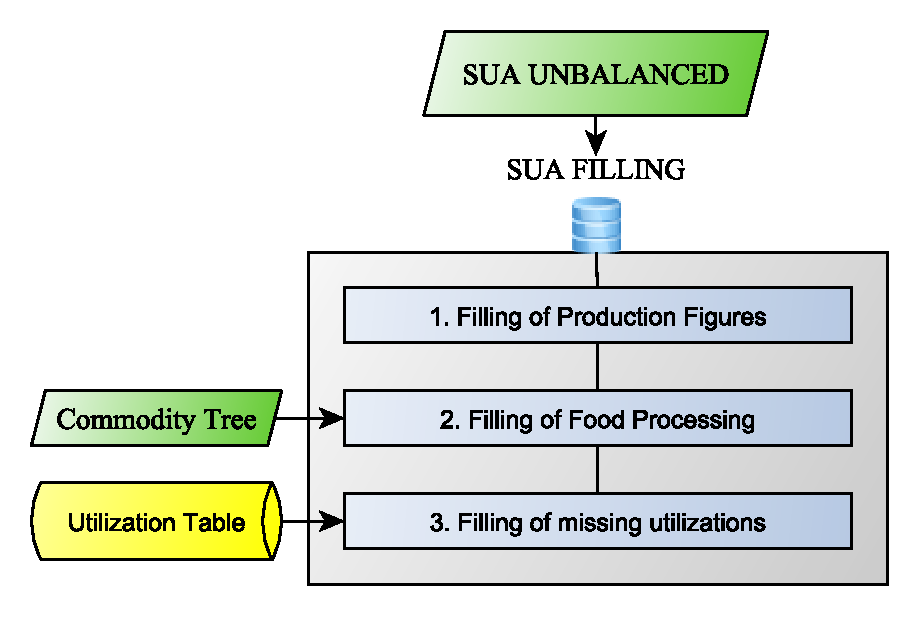
\includegraphics[width=0.6\linewidth]{images/StandBal/03b_suaFilling} 

}

\caption{\label{fig:f3}The Sua Filling simplified workflow}\label{fig:f3}
\end{figure}

\emph{Food Processing} needs to be computed first and it does not come
from any module. For the food processing to be correctly computed, a
check on the other variables has to be performed first, in order to be
sure that the food processing might be correctly imputed. In particular,
Production is checked first, as the \emph{Food Processing} figure of any
commodity is based on the production one. Then \emph{Food processing}
can be computed and, after that, other missing figures, if existing, are
filled.

This last step requires two major and not straightforward steps,
representing each a separate issue, for solving which, an algorithm has
been developed that responds to the following rationale and rules:

\begin{enumerate}
\def\labelenumi{\arabic{enumi}.}
\tightlist
\item
  \emph{Identify which are the missing values that have to be filled.}
\item
  \emph{Decide how to fill those missing values.}
\item
  \emph{Preserving reliability of sources of data}
\end{enumerate}

Not all the variables (supplies and Utilizations) are to be filled:

\begin{itemize}
\tightlist
\item
  Trade (import and Export) data are shared with countries and published
  by FAO. These figures have a separate process of validation that makes
  them reliable enough not to be questioned during the standardization
  process.
\item
  Production figures of primary commodities are also published by FAO.
  As previously mentioned, production values can have various flags
  which assign different degrees of reliability to these figures. The
  \emph{Sua Filling} treats production figures accordingly to flags.
\item
  \emph{Stock figures} are also very poor affected during the process of
  filling. This decision was taken because the standardization process
  works year by year, while \emph{stock variation} is a time-based
  variable that has to be always treated looking at the data over time.
  The cross year approach is incompatible with this characteristic. Any
  inconsistent or missing value for stock found would require to go back
  to the module imputing figures and check for possible errors. If no
  errors can be found, a manual correction would be required.
  Consequently these figures are never created from scratch, but might
  be sometimes reduced by a small percentage.
\end{itemize}

Information about the remaining variables, which are all Utilizations,
is taken from FBSs and SUAs of past years. FBSs published with the
previous methodology and their corresponding SUAs can give information
about which are the Utilizations supposed to be active for every single
commodity in each country.\\
These pieces of information have to be given externally, as the process
is automated and there is non-human knowledge intervening in training
the machine that is performing the calculations. The previous
methodology used for compiling FBS made massive use of manual
interventions while the new methodology tries to avoid it, but taking
advantage of the work and effort of the country experts that compiled
the FBSs in the past. Past information is embedded in the new
methodology through the use of the \emph{Utilization Table}. These table
helps identifying which variables have to be filled, commodity by
commodity. Moreover, the amount of them to be assigned to figures is
identified through a set of rules, known as \emph{Sua Filling}. This
procedure makes use of the imbalance between supply and utilization
values for each commodity and fills the figures that have been
recognized as missing from the \textbf{\emph{Utilization Table}}. The
filling procedure assigns figures using an ad-hoc algorithm, based on a
weight proportional to the size each variable had over the period
2000-2013, this size being represented by the median. As a consequence,
the majority of the commodities entering the \emph{Sua Filling}
procedure are eventually balanced.

Not all the commodities enter the process the same way. In particular, a
distinction is made between primary commodities, non-tree commodities
and derived commodities:

\begin{itemize}
\tightlist
\item
  Primary commodities are the commodities for which more reliable
  figures are produced. FAO often publishes information about primary
  commodities and a change of the figures has to be done with care.
\item
  Derived commodities are more affected by modifications during this
  process, according to the flag of each figure.
\item
  Non-Tree commodities (as previously defined) are treated as derived
  commodities.
\end{itemize}

Therefore, the steps of \emph{Sua Filling} process affect the SUA
differently from line to line. Figure \ref{fig:f4} shows the general
Workflow of the \emph{Sua Filling} highlighting the distinction between
primary and derived commodities.

\begin{figure}

{\centering \includegraphics[width=0.65\linewidth]{images/StandBal/04b_SuaFilling2} 

}

\caption{\label{fig:f4}The Sua Filling diversified workflow}\label{fig:f4}
\end{figure}

\subsection*{Step 1: Filling of production
figures}\label{step-1-filling-of-production-figures}
\addcontentsline{toc}{subsection}{Step 1: Filling of production figures}

Only Derived commodities are involved in this process. The \emph{Sua
Filling} detects the Production figures that need to be filled or
modified, by looking at the following \emph{Imbalance}:

\begin{equation}
\label{eq:imbalance1}
Imb1_{ijt} = P_{ijt} + I_{ijt} - X_{ijt}
\end{equation}

where \(Imb1_{ijt}\) is the Imbalance and is enumerated because is
different from a second Imbalance that will enter into the process
later. Here:

\begin{itemize}
\tightlist
\item
  If \(Imb1_{ijt} < 0\) there is no supply enough for the export and
  this is interpreted as the need for creating/increment the Production
  figure. The new production figure (\(P^*_{ijt}\)) is computed as:
\end{itemize}

\begin{equation}
\label{eq:imbalance1}
 P^*_{ijt} = P_{ijt} + Imb1_{ijt}
\end{equation}

\begin{itemize}
\tightlist
\item
  If \(Imb1_{ijt} >= 0\) there is enough supply and, therefore, no need
  for changing the production figure.
\end{itemize}

The reason for excluding other Variables from the computation of the
imbalance here is that, at this step of the process, Trade variables are
the most reliable and those for which, to the highest level of
probability, there are all the figures filled. In Table 3 \emph{Imb1} of
our example is reported. Notice that there are 3 rows with negative
values, one of which is a no-Tree commodity: \emph{Mixes and dough for
the preparation of baker's wares} (Table 4).

\begin{landscape}\begin{table}

\caption{\label{tab:t2}Sua table with Imb1 - China/Wheat/2014 example}
\centering
\resizebox{\linewidth}{!}{
\fontsize{18}{20}\selectfont
\begin{tabular}[t]{>{\raggedleft\arraybackslash}p{12em}|l|>{\raggedright\arraybackslash\leavevmode\color{black}}p{6em}|>{\raggedright\arraybackslash\leavevmode\color{black}}p{6em}|>{\raggedright\arraybackslash\leavevmode\color{black}}p{6em}|>{\raggedright\arraybackslash\leavevmode\color{black}}p{6em}|>{\raggedright\arraybackslash\leavevmode\color{black}}p{6em}|>{\raggedright\arraybackslash\leavevmode\color{black}}p{6em}|>{\raggedright\arraybackslash\leavevmode\color{black}}p{6em}|>{\raggedright\arraybackslash\leavevmode\color{black}}p{6em}|>{\raggedright\arraybackslash\leavevmode\color{black}}p{6em}|>{\raggedright\arraybackslash\leavevmode\color{black}}p{6em}|>{\raggedright\arraybackslash\leavevmode\color{black}}p{6em}|>{\bfseries\em\leavevmode\color{red}}l}
\hline
\multicolumn{1}{r}{\textbf{itemName}} & \multicolumn{1}{c}{\textbf{P}} & \multicolumn{1}{c}{\textbf{I}} & \multicolumn{1}{c}{\textbf{X}} & \multicolumn{1}{c}{\textbf{DSt}} & \multicolumn{1}{c}{\textbf{Fo}} & \multicolumn{1}{c}{\textbf{FP}} & \multicolumn{1}{c}{\textbf{Fe}} & \multicolumn{1}{c}{\textbf{Se}} & \multicolumn{1}{c}{\textbf{T}} & \multicolumn{1}{c}{\textbf{IU}} & \multicolumn{1}{c}{\textbf{L}} & \multicolumn{1}{c}{\textbf{ROU}} & \multicolumn{1}{c}{\textbf{Imb1}}\\
\hline
Wheat & 126,208,400 & 2,971,249 & 957 & 1,120,565 &  & - & 29,181,617 & 4,277,567 &  & 2,985,279 & 2,713,000 & - & 129,178,692\\
\hline
Wheat and meslin flo & 70,500,000 & 33,055 & 188,674 &  & 67,300,000 & - &  &  & -17,345 &  &  & - & 70,344,381\\
\hline
Mixes and doughs for &  & 6,497 & 38,072 &  & 0 & - & 0 &  & 0 &  &  & - & -31,575\\
\hline
Other Fructose and S & 126,277 & 3,659 & 162,324 &  & 0 & - &  &  & 0 &  &  & - & -32,388\\
\hline
Starch of Wheat & 239,816 & 11,035 & 40,311 &  &  & - & 172,196 &  &  & 7,919 &  & - & 210,541\\
\hline
Wheat Gluten & 25,580 & 877 & 117,373 &  &  & - & 0 &  &  &  &  & - & -90,916\\
\hline
Communion wafers & 13,263 & 8,796 & 5,822 &  & 16,241 & - &  &  & -4 &  &  & - & 16,237\\
\hline
Uncooked pasta & 1,415,692 & 12,520 & 22,550 &  & 1,405,661 & - &  &  & -362 &  &  & - & 1,405,661\\
\hline
Food Preparations of &  & 69,686 & 21,977 &  & 47,709 & - &  &  & -12 &  &  & - & 47,709\\
\hline
Bran of Wheat & 21,414,279 & 156,359 & 2,200 &  & 16,500,000 & - & 4,827,244 &  & -4,252 &  &  & - & 21,568,438\\
\hline
Gluten Feed and Meal & 793,740 & 160,231 & 529,333 &  &  & - &  &  &  &  &  & - & 424,638\\
\hline
bread & 15,485 & 2,897 & 4,210 &  & 14,175 & - &  &  & -3 &  &  & - & 14,172\\
\hline
pastry & 193,950 & 89,593 & 117,630 &  & 165,914 & - &  &  & -43 &  &  & - & 165,914\\
\hline
\multicolumn{14}{l}{\textsuperscript{a} P=Production, I=Import, X=Export, DSt=Delta Stock, Fo=Food Availability, FP=FoodProcessing, Fe=Feed, Se=Seed, T=Tourism Consumption, IU=IndustrialUse, L=Loss, ROU=Residual and other uses}\\
\end{tabular}}
\end{table}
\end{landscape}

\begin{landscape}\begin{table}

\caption{\label{tab:t3}Sua table with Production filled/incremented - China/Wheat/2014 example}
\centering
\resizebox{\linewidth}{!}{
\fontsize{18}{20}\selectfont
\begin{tabular}[t]{>{\raggedleft\arraybackslash}p{12em}|l|>{\raggedright\arraybackslash\leavevmode\color{black}}p{6em}|>{\raggedright\arraybackslash\leavevmode\color{black}}p{6em}|>{\raggedright\arraybackslash\leavevmode\color{black}}p{6em}|>{\raggedright\arraybackslash\leavevmode\color{black}}p{6em}|>{\raggedright\arraybackslash\leavevmode\color{black}}p{6em}|>{\raggedright\arraybackslash\leavevmode\color{black}}p{6em}|>{\raggedright\arraybackslash\leavevmode\color{black}}p{6em}|>{\raggedright\arraybackslash\leavevmode\color{black}}p{6em}|>{\raggedright\arraybackslash\leavevmode\color{black}}p{6em}|>{\raggedright\arraybackslash\leavevmode\color{black}}p{6em}|>{\raggedright\arraybackslash\leavevmode\color{black}}p{6em}|>{\raggedright\arraybackslash\leavevmode\color{black}}p{6em}}
\hline
\multicolumn{1}{r}{\textbf{itemName}} & \multicolumn{1}{c}{\textbf{P}} & \multicolumn{1}{c}{\textbf{I}} & \multicolumn{1}{c}{\textbf{X}} & \multicolumn{1}{c}{\textbf{DSt}} & \multicolumn{1}{c}{\textbf{Fo}} & \multicolumn{1}{c}{\textbf{FP}} & \multicolumn{1}{c}{\textbf{Fe}} & \multicolumn{1}{c}{\textbf{Se}} & \multicolumn{1}{c}{\textbf{T}} & \multicolumn{1}{c}{\textbf{IU}} & \multicolumn{1}{c}{\textbf{L}} & \multicolumn{1}{c}{\textbf{ROU}} & \multicolumn{1}{c}{\textbf{Imb1}}\\
\hline
Wheat & 126,208,400 & 2,971,249 & 957 & 1,120,565 &  & - & 29,181,617 & 4,277,567 &  & 2,985,279 & 2,713,000 & - & 129,178,692\\
\hline
Wheat and meslin flo & 70,500,000 & 33,055 & 188,674 &  & 67,300,000 & - &  &  & -17,345 &  &  & - & 70,344,381\\
\hline
\textcolor{red}{\em{\textbf{Mixes and doughs for}}} & \textcolor{red}{\em{\textbf{**31,575**}}} & \textcolor{red}{\em{\textbf{6,497}}} & \textcolor{red}{\em{\textbf{38,072}}} & \textcolor{red}{\em{\textbf{}}} & \textcolor{red}{\em{\textbf{0}}} & \textcolor{red}{\em{\textbf{-}}} & \textcolor{red}{\em{\textbf{0}}} & \textcolor{red}{\em{\textbf{}}} & \textcolor{red}{\em{\textbf{0}}} & \textcolor{red}{\em{\textbf{}}} & \textcolor{red}{\em{\textbf{}}} & \textcolor{red}{\em{\textbf{-}}} & \textcolor{red}{\em{\textbf{0}}}\\
\hline
\textcolor{red}{\em{\textbf{Other Fructose and S}}} & \textcolor{red}{\em{\textbf{**158,665**}}} & \textcolor{red}{\em{\textbf{3,659}}} & \textcolor{red}{\em{\textbf{162,324}}} & \textcolor{red}{\em{\textbf{}}} & \textcolor{red}{\em{\textbf{0}}} & \textcolor{red}{\em{\textbf{-}}} & \textcolor{red}{\em{\textbf{}}} & \textcolor{red}{\em{\textbf{}}} & \textcolor{red}{\em{\textbf{0}}} & \textcolor{red}{\em{\textbf{}}} & \textcolor{red}{\em{\textbf{}}} & \textcolor{red}{\em{\textbf{-}}} & \textcolor{red}{\em{\textbf{0}}}\\
\hline
Starch of Wheat & 239,816 & 11,035 & 40,311 &  &  & - & 172,196 &  &  & 7,919 &  & - & 210,541\\
\hline
\textcolor{red}{\em{\textbf{Wheat Gluten}}} & \textcolor{red}{\em{\textbf{**116,496**}}} & \textcolor{red}{\em{\textbf{877}}} & \textcolor{red}{\em{\textbf{117,373}}} & \textcolor{red}{\em{\textbf{}}} & \textcolor{red}{\em{\textbf{}}} & \textcolor{red}{\em{\textbf{-}}} & \textcolor{red}{\em{\textbf{0}}} & \textcolor{red}{\em{\textbf{}}} & \textcolor{red}{\em{\textbf{}}} & \textcolor{red}{\em{\textbf{}}} & \textcolor{red}{\em{\textbf{}}} & \textcolor{red}{\em{\textbf{-}}} & \textcolor{red}{\em{\textbf{0}}}\\
\hline
Communion wafers & 13,263 & 8,796 & 5,822 &  & 16,241 & - &  &  & -4 &  &  & - & 16,237\\
\hline
Uncooked pasta & 1,415,692 & 12,520 & 22,550 &  & 1,405,661 & - &  &  & -362 &  &  & - & 1,405,661\\
\hline
Food Preparations of &  & 69,686 & 21,977 &  & 47,709 & - &  &  & -12 &  &  & - & 47,709\\
\hline
Bran of Wheat & 21,414,279 & 156,359 & 2,200 &  & 16,500,000 & - & 4,827,244 &  & -4,252 &  &  & - & 21,568,438\\
\hline
Gluten Feed and Meal & 793,740 & 160,231 & 529,333 &  &  & - &  &  &  &  &  & - & 424,638\\
\hline
bread & 15,485 & 2,897 & 4,210 &  & 14,175 & - &  &  & -3 &  &  & - & 14,172\\
\hline
pastry & 193,950 & 89,593 & 117,630 &  & 165,914 & - &  &  & -43 &  &  & - & 165,914\\
\hline
\multicolumn{14}{l}{\textsuperscript{a} P=Production, I=Import, X=Export, DSt=Delta Stock, Fo=Food Availability, FP=FoodProcessing, Fe=Feed, Se=Seed, T=Tourism Consumption, IU=IndustrialUse, L=Loss, ROU=Residual and other uses}\\
\multicolumn{14}{l}{\textsuperscript{b} Starred figures are those that have changed from the previous table}\\
\end{tabular}}
\end{table}
\end{landscape}

\subsection*{Step 2: Filling of food
processing}\label{step-2-filling-of-food-processing}
\addcontentsline{toc}{subsection}{Step 2: Filling of food processing}

When Production has been checked, created or incremented, \emph{Food
Processing} can be calculated. Food processing is the amount of the
supply of a commodity processed into derived commodities. \emph{Food
processing} is calculated for all the parent commodities as the sum of
the food processing of all the possible derived commodities. For
example, Wheat in China is processed into Flour of Wheat, Bran of Wheat
and Breakfast Cereals. Flour and Bran are produced during the same
production process (they are called \emph{co-products} or
\emph{by-products}), meaning that the same amount of wheat is used for
producing all of them. Breakfast Cereals comes from a separate
production process instead. Therefore, \emph{Food processing} of Wheat
is given as the sum of the amount of wheat's supply used for producing
Flour and Bran + The amount used for producing Breakfast Cereals.
Calculation of Food processing happens by level, then after having
calculated the amount for wheat, the amount of supply of flour of wheat
used for producing Starch, Gluten, bread and the other derived of wheat
flour becomes the \emph{Food processing} of flour of Wheat and so on,
for any subsequent level.

The formula for calculating \(FP\) is based on the production of the
child product:

\begin{equation}
\label{eq:Food Processing}
FP_{pjt} = \sum \limits_{c=1}^C\biggl(\frac{P_{cjt}}{eR_{p\to c}}\biggr)\times s^{1}_{cp}\times w_{c}
\end{equation}

where:

\begin{itemize}
\tightlist
\item
  \(FP_{pjt}\) is \emph{Food processing} of the generic parent \(p\).
\item
  \(c = 1,2,3...C\) are the \(C\) children \(c\) of parent \(p\).
\item
  \(P_{cjt}\) is the Production of Child \(c\).
\item
  \(eR_{p\to c}\) is the \emph{extraction Rate} from parent \(p\) to
  child \(c\).
\item
  \(s^{1}_{cp}\) is the \emph{share} of child \(c\) from parent \(p\)
  specific for Food Processing calculation. It is defined as:
\end{itemize}

\begin{quote}
\begin{equation}
\label{eq:shares}
s^{1}_{cp} = \frac{availability1_{p(c)}}{\sum \limits_{p=1}^A{availability1_{p(c)}}}
\end{equation}
\end{quote}

\begin{quote}
where \(availability1_{p(c)}\) is the availability of each parent \(p\)
of child \(c\) expressed in terms of \(c\) (as say in \emph{child
equivalent}). Is is enumerated as \(1\) because a slighlty different
availability will be found in a following step:
\end{quote}

\begin{quote}
\begin{quote}
\begin{equation}
\label{eq:availability 1}
availability1_{p(c)} = (P_{pjt} + I_{pjt} - X_{pjt})\times eR_{p\to c}
\end{equation}
\end{quote}
\end{quote}

\begin{itemize}
\tightlist
\item
  \(w_{c}\) is the \emph{weight} of child \(c\). This parameter is used
  for identifying and treating co-products. Indeed, if the production of
  two or more co-products is used for producing \emph{Food processing}
  of the parent commodity producing them, the result would be a Food
  processing twice the size of what it should be. This would happen
  because the two co-products are produced during the same process, from
  the same amount of the parent commodity. For this to be taken into
  account, a weight is used, which is 1 for the commodity that has to be
  considered for determining Food processing of parent commodity and 0
  for the child commodities that are co-products (equation
  \ref{eq:weight}). Please notice that, the co-products are still
  important in the standardization, because they contribute in the
  creation of the calories availability of the country. These
  commodities (Also called \emph{zero weight} commodities) are
  multiplied by 0 only when quantities are treated, they will instead be
  considered when calories will be taken into account:
\end{itemize}

\begin{quote}
\begin{quote}
\begin{equation}
\label{eq:weight}
\begin{cases}
w_{c} = 1      & \quad \text{if both quantity and calories have to be standardized} \\
w_{c} = 0      & \quad \text{if only calories have to be standardized}
\end{cases}
\end{equation}
\end{quote}
\end{quote}

The following Table reports the commodity tree of the
\emph{China/Wheat/2014} example with the extra-column reporting the
\emph{weight} of each child-commodity.

\begin{table}

\caption{\label{tab:t4}Commodity Tree  with weights - China/Wheat/2014 example}
\centering
\begin{tabular}[t]{r|l|l|l|l|l|l}
\hline
Country & Year & ParentName & ChildName & eR & share & weight\\
\hline
China, Mainland & 2014 & Wheat & Wheat and meslin flo & 0.78 & 1.00 & 1\\
\hline
China, Mainland & 2014 & Wheat & Bran of Wheat & 0.22 & 1.00 & 0\\
\hline
China, Mainland & 2014 & Wheat and meslin flo & Uncooked pasta, not & 1.00 & 1.00 & 1\\
\hline
China, Mainland & 2014 & Wheat and meslin flo & bread & 1.00 & 1.00 & 1\\
\hline
China, Mainland & 2014 & Wheat and meslin flo & pastry & 1.00 & 1.00 & 1\\
\hline
China, Mainland & 2014 & Wheat and meslin flo & Starch of Wheat & 0.75 & 1.00 & 1\\
\hline
China, Mainland & 2014 & Wheat and meslin flo & Wheat Gluten & 0.08 & 1.00 & 0\\
\hline
China, Mainland & 2014 & Wheat and meslin flo & Communion wafers, em & 1.00 & 1.00 & 1\\
\hline
China, Mainland & 2014 & Starch of Wheat & Other Fructose and S & 1.00 & 1.00 & 1\\
\hline
China, Mainland & 2014 & Wheat Gluten & Gluten Feed and Meal & 1.00 & 0.33 & 1\\
\hline
China, Mainland & 2014 & Bran of Maize & Gluten Feed and Meal & 1.00 & 0.67 & 1\\
\hline
\end{tabular}
\end{table}

Shares lower than \(1\) mean that the child commodity might be produced
also from other parents and the reported ratio represents the ratio of
that commodity that is produced from the reported parent. For example,
\emph{Gluten Feed and Meal} is produced from \emph{Wheat Gluten} and
from \emph{Bran of maize}. The sum of the shares associated to this
child (\(0.33\) and \(0.67\)) is equal to \(1\).

Table 6 shows the SUA table after the two steps just described. Notice
that, in the specific example, there was no need for the
creation/increase of Production on any derived commodity because
\(Imb1\) is positive for all commodities.

From Table 5 and Table 6 here is, as example, the computation of
\emph{Food processing} of Wheat,Flour of wheat and Starch of wheat:

\begin{equation}
\begin{multlined}
\label{eq:wheatFP}
FP_{wheatChina2014} = \left(70,500,000/0.78\right)\times 1\times 1 +\left(21,414,729/0.8\right)\times 1\times 0 = 90,384,615
\end{multlined}
\end{equation}

\begin{equation}
\begin{multlined}
\label{eq:flourFP}
FP_{flourChina2014} = \left(1,415,692/1\right)\times 1\times 1 +\left(15,486/1\right)\times 1\times 1 
+\left(193,950/1\right)\times 1\times 1
+\\
\left(239,816/0.75\right)\times 1\times 1 +
\left(116,496/1\right)\times 1\times 0 +\left(13,263/1\right)\times 1\times 1= 1,958,146
\end{multlined}
\end{equation}

\begin{equation}
\begin{multlined}
\label{eq:starchFP}
FP_{starchChina2014} = \left(158,665/1\right)\times 1\times 1 +\left(21,414,729/0.8\right)\times 1\times 0 = 158,665
\end{multlined}
\end{equation}

\begin{landscape}\begin{table}

\caption{\label{tab:t5}Sua table with Food Processing filled - China/Wheat/2014 example}
\centering
\resizebox{\linewidth}{!}{
\fontsize{18}{20}\selectfont
\begin{tabular}[t]{>{\raggedleft\arraybackslash}p{12em}|>{\raggedright\arraybackslash}p{6em}|>{\raggedright\arraybackslash}p{6em}|>{\raggedright\arraybackslash}p{6em}|>{\raggedright\arraybackslash}p{6em}|>{\raggedright\arraybackslash}p{6em}|>{\bfseries\em\leavevmode\color{red}}l|>{\raggedright\arraybackslash}p{6em}|>{\raggedright\arraybackslash}p{6em}|>{\raggedright\arraybackslash}p{6em}|>{\raggedright\arraybackslash}p{6em}|>{\raggedright\arraybackslash}p{6em}|>{\raggedright\arraybackslash}p{6em}}
\hline
\multicolumn{1}{r}{\textbf{itemName}} & \multicolumn{1}{c}{\textbf{P}} & \multicolumn{1}{c}{\textbf{I}} & \multicolumn{1}{c}{\textbf{X}} & \multicolumn{1}{c}{\textbf{DSt}} & \multicolumn{1}{c}{\textbf{Fo}} & \multicolumn{1}{c}{\textbf{FP}} & \multicolumn{1}{c}{\textbf{Fe}} & \multicolumn{1}{c}{\textbf{Se}} & \multicolumn{1}{c}{\textbf{T}} & \multicolumn{1}{c}{\textbf{IU}} & \multicolumn{1}{c}{\textbf{L}} & \multicolumn{1}{c}{\textbf{ROU}}\\
\hline
Wheat & 126,208,400 & 2,971,249 & 957 & 1,120,565 &  & **90,384,615** & 29,181,617 & 4,277,567 &  & 2,985,279 & 2,713,000 & -\\
\hline
Wheat and meslin flo & 70,500,000 & 33,055 & 188,674 &  & 67,300,000 & **1,958,146** &  &  & -17,345 &  &  & -\\
\hline
Mixes and doughs for & 31,575 & 6,497 & 38,072 &  & 0 &  & 0 &  & 0 &  &  & -\\
\hline
Other Fructose and S & 158,665 & 3,659 & 162,324 &  & 0 &  &  &  & 0 &  &  & -\\
\hline
Starch of Wheat & 239,816 & 11,035 & 40,311 &  &  & **158,664** & 172,196 &  &  & 7,919 &  & -\\
\hline
Wheat Gluten & 116,496 & 877 & 117,373 &  &  & **264,580** & 0 &  &  &  &  & -\\
\hline
Communion wafers & 13,263 & 8,796 & 5,822 &  & 16,241 &  &  &  & -4 &  &  & -\\
\hline
Uncooked pasta & 1,415,692 & 12,520 & 22,550 &  & 1,405,661 &  &  &  & -362 &  &  & -\\
\hline
Food Preparations of &  & 69,686 & 21,977 &  & 47,709 &  &  &  & -12 &  &  & -\\
\hline
Bran of Wheat & 21,414,279 & 156,359 & 2,200 &  & 16,500,000 &  & 4,827,244 &  & -4,252 &  &  & -\\
\hline
Gluten Feed and Meal & 793,740 & 160,231 & 529,333 &  &  &  &  &  &  &  &  & -\\
\hline
bread & 15,485 & 2,897 & 4,210 &  & 14,175 &  &  &  & -3 &  &  & -\\
\hline
pastry & 193,950 & 89,593 & 117,630 &  & 165,914 &  &  &  & -43 &  &  & -\\
\hline
\multicolumn{13}{l}{\textsuperscript{a} P=Production, I=Import, X=Export, DSt=Delta Stock, Fo=Food Availability, FP=FoodProcessing, Fe=Feed, Se=Seed, T=Tourism Consumption, IU=IndustrialUse, L=Loss, ROU=Residual and other uses}\\
\multicolumn{13}{l}{\textsuperscript{b} Starred figures are those that have changed from the previous table}\\
\end{tabular}}
\end{table}
\end{landscape}

\subsection*{Step 3: Filling of other missing
Utilizations}\label{step-3-filling-of-other-missing-utilizations}
\addcontentsline{toc}{subsection}{Step 3: Filling of other missing
Utilizations}

After \emph{Food processing} figures have been computed, the other
variables have to be checked and either filled, increased or decreased.
This step is based on the value of the following Imbalance:

\begin{equation}
\label{eq:imbalance2}
Imb2_{ijt} = P_{ijt} + I_{ijt} - X_{ijt} - \Delta St_{ijt} - FP_{ijt} - Fo_{ijt} - Fe_{ijt} - Lo_{ijt} - Se_{ijt} - IU_{ijt} - T_{ijt}
\end{equation}

Table 7 reports \(Imb2\) for all the lines of the SUAs of our example.

Three different scenarios con be found (Figure 5):

\begin{figure}

{\centering 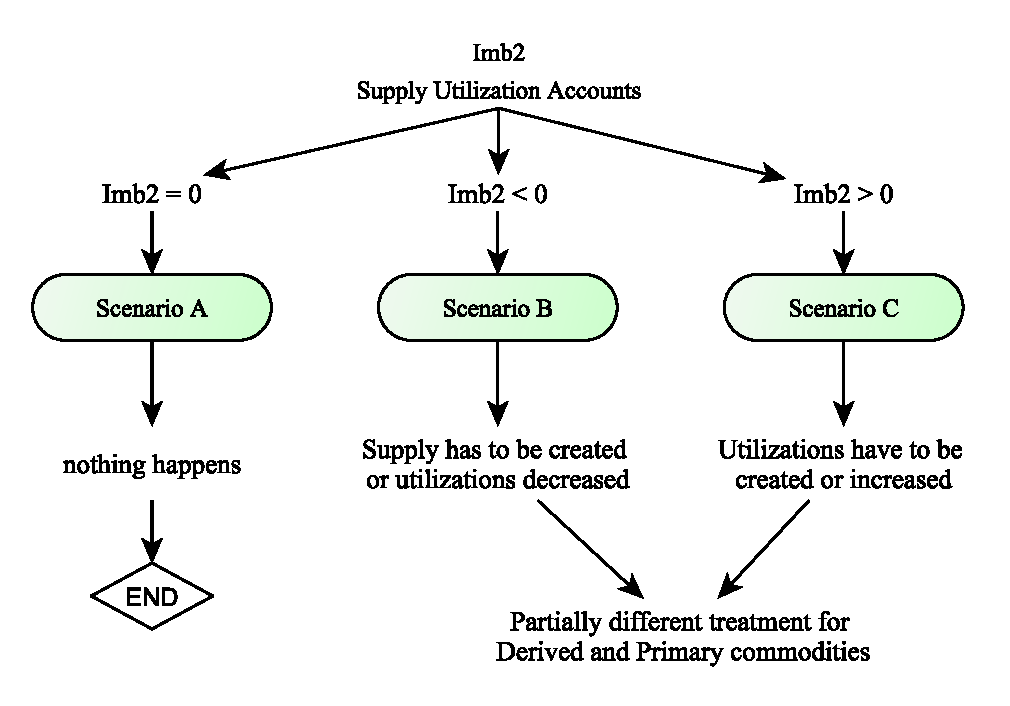
\includegraphics[width=0.8\linewidth]{images/StandBal/05b_ScenariosFilling} 

}

\caption{\label{fig:f5}Scenarios of the Sua Filling}\label{fig:f5}
\end{figure}

\begin{landscape}\begin{table}

\caption{\label{tab:t6}Sua table with Imb2 - China/Wheat/2014 example}
\centering
\resizebox{\linewidth}{!}{
\fontsize{18}{20}\selectfont
\begin{tabular}[t]{>{\raggedleft\arraybackslash}p{10em}|l|>{\raggedright\arraybackslash\leavevmode\color{black}}p{6em}|>{\raggedright\arraybackslash\leavevmode\color{black}}p{6em}|>{\raggedright\arraybackslash\leavevmode\color{black}}p{6em}|>{\raggedright\arraybackslash\leavevmode\color{black}}p{6em}|>{\raggedright\arraybackslash\leavevmode\color{black}}p{6em}|>{\raggedright\arraybackslash\leavevmode\color{black}}p{6em}|>{\raggedright\arraybackslash\leavevmode\color{black}}p{6em}|>{\raggedright\arraybackslash\leavevmode\color{black}}p{6em}|>{\raggedright\arraybackslash\leavevmode\color{black}}p{6em}|>{\raggedright\arraybackslash\leavevmode\color{black}}p{6em}|>{\raggedright\arraybackslash\leavevmode\color{black}}p{6em}|>{\bfseries\em\leavevmode\color{red}}l}
\hline
\multicolumn{1}{r}{\textbf{itemName}} & \multicolumn{1}{c}{\textbf{P}} & \multicolumn{1}{c}{\textbf{I}} & \multicolumn{1}{c}{\textbf{X}} & \multicolumn{1}{c}{\textbf{DSt}} & \multicolumn{1}{c}{\textbf{Fo}} & \multicolumn{1}{c}{\textbf{FP}} & \multicolumn{1}{c}{\textbf{Fe}} & \multicolumn{1}{c}{\textbf{Se}} & \multicolumn{1}{c}{\textbf{T}} & \multicolumn{1}{c}{\textbf{IU}} & \multicolumn{1}{c}{\textbf{L}} & \multicolumn{1}{c}{\textbf{ROU}} & \multicolumn{1}{c}{\textbf{Imb2}}\\
\hline
Wheat & 126,208,400 & 2,971,249 & 957 & 1,120,565 &  & 90,384,615 & 29,181,617 & 4,277,567 &  & 2,985,279 & 2,713,000 & - & -1,483,951\\
\hline
Wheat and meslin flo & 70,500,000 & 33,055 & 188,674 &  & 67,300,000 & 1,958,146 &  &  & -17,345 &  &  & - & 1,103,580\\
\hline
Mixes and doughs for & 31,575 & 6,497 & 38,072 &  & 0 &  & 0 &  & 0 &  &  & - & -31,575\\
\hline
Other Fructose and S & 158,665 & 3,659 & 162,324 &  & 0 &  &  &  & 0 &  &  & - & 0\\
\hline
Starch of Wheat & 239,816 & 11,035 & 40,311 &  &  & 158,664 & 172,196 &  &  & 7,919 &  & - & -128,239\\
\hline
Wheat Gluten & 116,496 & 877 & 117,373 &  &  & 264,580 & 0 &  &  &  &  & - & -264,580\\
\hline
Communion wafers & 13,263 & 8,796 & 5,822 &  & 16,241 &  &  &  & -4 &  &  & - & 0\\
\hline
Uncooked pasta & 1,415,692 & 12,520 & 22,550 &  & 1,405,661 &  &  &  & -362 &  &  & - & 363\\
\hline
Food Preparations of &  & 69,686 & 21,977 &  & 47,709 &  &  &  & -12 &  &  & - & 12\\
\hline
Bran of Wheat & 21,414,279 & 156,359 & 2,200 &  & 16,500,000 &  & 4,827,244 &  & -4,252 &  &  & - & 245,447\\
\hline
Gluten Feed and Meal & 793,740 & 160,231 & 529,333 &  &  &  &  &  &  &  &  & - & 424,638\\
\hline
bread & 15,485 & 2,897 & 4,210 &  & 14,175 &  &  &  & -3 &  &  & - & 0\\
\hline
pastry & 193,950 & 89,593 & 117,630 &  & 165,914 &  &  &  & -43 &  &  & - & 42\\
\hline
\multicolumn{14}{l}{\textsuperscript{a} P=Production, I=Import, X=Export, DSt=Delta Stock, Fo=Food Availability, FP=FoodProcessing, Fe=Feed, Se=Seed, T=Tourism Consumption, IU=IndustrialUse, L=Loss, ROU=Residual and other uses}\\
\end{tabular}}
\end{table}
\end{landscape}

\subsubsection*{\texorpdfstring{\emph{Imbalance = 0 (Scenario
A)}}{Imbalance = 0 (Scenario A)}}\label{imbalance-0-scenario-a}
\addcontentsline{toc}{subsubsection}{\emph{Imbalance = 0 (Scenario A)}}

In this scenario, the Imbalance is null, this meaning that there is
enough supply for the existing utilization. In this case, the SUA line
is balanced and nothing happens for the commodity. In Table 7 this is
the case of \emph{Other Fructose and syrup} and \emph{wheat Gluten}.

\subsubsection*{\texorpdfstring{\emph{Imbalance \textless{} 0 (Scenario
B)}}{Imbalance \textless{} 0 (Scenario B)}}\label{imbalance-0-scenario-b}
\addcontentsline{toc}{subsubsection}{\emph{Imbalance \textless{} 0
(Scenario B)}}

If this happens, it means that there is not enough supply for the
commodity to be used in the way the SUA figures suggest. In this case,
as shown in Figure \ref{fig:f6} the algorithm tries to solve the excess
of utilization by reducing all the existing Utilizations by 30\% (except
Exports (Stock is changed in this case, because this is just a
proportional reduction of values and does not need a time series
analysis).

All commodities enter this step, Primary commodity included.

If this is enough to cover the Utilization, the balancing line for that
commodity is balanced and the process can go to the next step. Instead,
after this reduction, there might be 2 different scenarios:

\begin{enumerate}
\def\labelenumi{\arabic{enumi}.}
\tightlist
\item
  If this imbalance is still negative, Primary commodities remain
  unbalanced, while derived commodities can be still changed. In this
  case it is checked if the production figure is ``\emph{protected}'' or
  not:
\end{enumerate}

\begin{quote}
-- If Production figure is not protected, it is interpreted as if there
was not enough information for producing a correct production
number.This figure is then changed, i.e.~created, if missing, or
incremented of an amount equal to \emph{Imb2}
\end{quote}

\begin{quote}
-- If Production figure is protected, a warning is given that tells that
there is an unsolvable problem and that all figures have to be checked
because either the production protected figure is wrong, or the Trade or
some utilization have to be changed.
\end{quote}

\begin{enumerate}
\def\labelenumi{\arabic{enumi}.}
\setcounter{enumi}{1}
\tightlist
\item
  If the imbalance becomes positive, the line (in all cases, derived or
  primary commodities) falls into the Scenario C that will be explained
  shortly.
\end{enumerate}

\emph{Starch of Wheat} belongs to this very last case. Indeed, it has a
negative Imbalance, therefore, its Utilizations are reduced by 30\% of
their values (see Table 8). After that happens, the Imb2 is recalculated
and it is still negative, equal to \(74,204\) (this value is not
reported in the table). In the following step, as the production is not
protected, the new value of production is equal to:

\begin{equation}
\label{eq:prod}
P_{StarchChina2014} = 239,816 + 74,204 = 314,020
\end{equation}

Notice that, after this step, all commodities are balanced.

\begin{figure}

{\centering 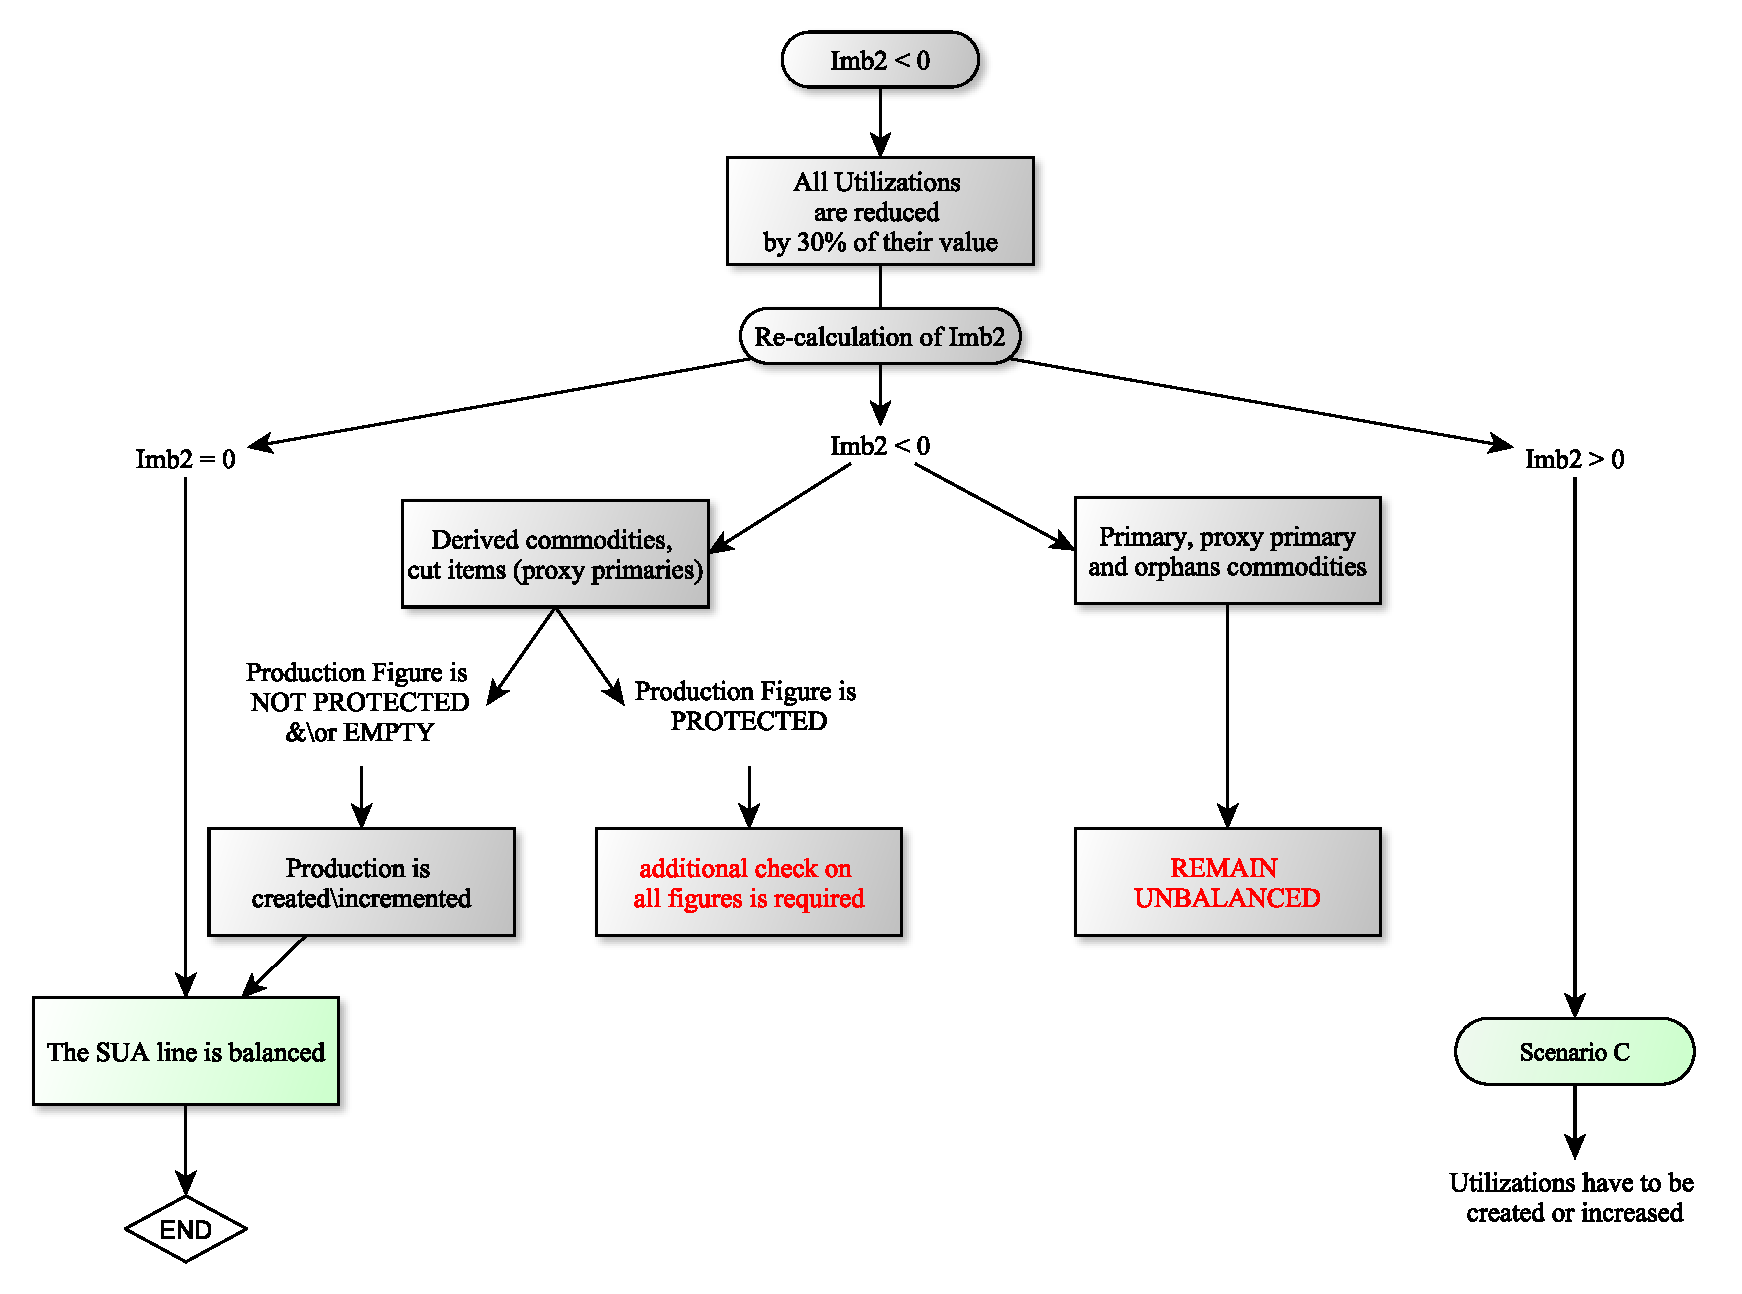
\includegraphics{images/StandBal/06b_NegativeImbalance} 

}

\caption{\label{fig:f5}Workflow of Sua Filling when there is a negative imbalance}\label{fig:f6}
\end{figure}

\begin{landscape}\begin{table}

\caption{\label{tab:t7}Sua table with Utilizations filled - China/Wheat/2014 example}
\centering
\resizebox{\linewidth}{!}{
\fontsize{18}{20}\selectfont
\begin{tabular}[t]{>{\raggedleft\arraybackslash}p{10em}|l|>{\raggedright\arraybackslash\leavevmode\color{black}}p{6em}|>{\raggedright\arraybackslash\leavevmode\color{black}}p{6em}|>{\raggedright\arraybackslash\leavevmode\color{black}}p{6em}|>{\raggedright\arraybackslash\leavevmode\color{black}}p{6em}|>{\raggedright\arraybackslash\leavevmode\color{black}}p{6em}|>{\raggedright\arraybackslash\leavevmode\color{black}}p{6em}|>{\raggedright\arraybackslash\leavevmode\color{black}}p{6em}|>{\raggedright\arraybackslash\leavevmode\color{black}}p{6em}|>{\raggedright\arraybackslash\leavevmode\color{black}}p{6em}|>{\raggedright\arraybackslash\leavevmode\color{black}}p{6em}|>{\raggedright\arraybackslash\leavevmode\color{black}}p{6em}|>{\bfseries\em\leavevmode\color{red}}l}
\hline
\multicolumn{1}{r}{\textbf{itemName}} & \multicolumn{1}{c}{\textbf{P}} & \multicolumn{1}{c}{\textbf{I}} & \multicolumn{1}{c}{\textbf{X}} & \multicolumn{1}{c}{\textbf{DSt}} & \multicolumn{1}{c}{\textbf{Fo}} & \multicolumn{1}{c}{\textbf{FP}} & \multicolumn{1}{c}{\textbf{Fe}} & \multicolumn{1}{c}{\textbf{Se}} & \multicolumn{1}{c}{\textbf{T}} & \multicolumn{1}{c}{\textbf{IU}} & \multicolumn{1}{c}{\textbf{L}} & \multicolumn{1}{c}{\textbf{ROU}} & \multicolumn{1}{c}{\textbf{Imb2}}\\
\hline
Wheat & 126,208,400 & 2,971,249 & 957 & **1,079,280** &  & 90,384,615 & **28,106,487** & **4,119,970** &  & **2,875,293** & **2,613,046** & - & 0\\
\hline
Wheat and meslin flo & 70,500,000 & 33,055 & 188,674 &  & **68,372,646** & 1,958,146 &  &  & **-17,621** &  &  & - & 0\\
\hline
Mixes and doughs for & 31,575 & 6,497 & 38,072 &  & 0 &  & 0 &  & 0 &  &  & - & 0\\
\hline
Other Fructose and S & 158,665 & 3,659 & 162,324 &  & 0 &  &  &  & 0 &  &  & - & 0\\
\hline
Starch of Wheat & **314,020** & 11,035 & 40,311 &  &  & 158,664 & **120,537** &  &  & **5,543** &  & - & 0\\
\hline
Wheat Gluten & **381,076** & 877 & 117,373 &  &  & 264,580 & 0 &  &  &  &  & - & 0\\
\hline
Communion wafers & 13,263 & 8,796 & 5,822 &  & 16,241 &  &  &  & -4 &  &  & - & 0\\
\hline
Uncooked pasta & 1,415,692 & 12,520 & 22,550 &  & **1,406,024** &  &  &  & **-363** &  &  & - & 0\\
\hline
Food Preparations of &  & 69,686 & 21,977 &  & **47,721** &  &  &  & -12 &  &  & - & 0\\
\hline
Bran of Wheat & 21,414,279 & 156,359 & 2,200 &  & **16,689,929** &  & **4,882,810** &  & **-4,301** &  &  & - & 0\\
\hline
Gluten Feed and Meal & 793,740 & 160,230 & 529,333 &  &  &  & **424,637** &  &  &  &  & - & 0\\
\hline
bread & 15,485 & 2,897 & 4,210 &  & 14,175 &  &  &  & -3 &  &  & - & 0\\
\hline
pastry & 193,950 & 89,593 & 117,630 &  & **165,957** &  &  &  & **-42.75** &  &  & - & 0\\
\hline
\multicolumn{14}{l}{\textsuperscript{a} P=Production, I=Import, X=Export, DSt=Delta Stock, Fo=Food Availability, FP=FoodProcessing, Fe=Feed, Se=Seed, T=Tourism Consumption, IU=IndustrialUse, L=Loss, ROU=Residual and other uses}\\
\multicolumn{14}{l}{\textsuperscript{b} Starred figures are those that have changed from the previous table}\\
\end{tabular}}
\end{table}
\end{landscape}

\subsubsection*{\texorpdfstring{\emph{Imbalance \textgreater{} 0
(Scenario
C)}}{Imbalance \textgreater{} 0 (Scenario C)}}\label{imbalance-0-scenario-c}
\addcontentsline{toc}{subsubsection}{\emph{Imbalance \textgreater{} 0
(Scenario C)}}

When \(Imb2 >0\) there is an excess of supply that has to be distributed
through Utilizations. Here:

\begin{itemize}
\tightlist
\item
  A \emph{Utilization Table} tells which figures are supposed to be
  filled.
\item
  The Imbalance is distributed among variables according to a, so
  called, \emph{Multiple Filler approach} that distributes imbalance
  according to weights proportional to median values of variables over a
  time ange (2000-2013).
\end{itemize}

\subsubsection*{\texorpdfstring{--\textgreater{} The \emph{Utilization
Table}}{--\textgreater{} The Utilization Table}}\label{the-utilization-table}
\addcontentsline{toc}{subsubsection}{--\textgreater{} The
\emph{Utilization Table}}

\emph{Utilization Table} is a Country/commodity table telling which
Utilizations historically have been active for each commodity and
assigning a Rank and an inverse rank to each utilization based on its
mean value over the period 2000-2013. Table 9 shows the
\emph{Utilization Table} for \emph{Wheat and meslin flour} in China
Mainland.

\begin{table}

\caption{\label{tab:t8}*Utilization Table* Wheat and meslin Flour - China/Wheat/2014 example}
\centering
\begin{tabular}[t]{c|c|c|c|c}
\hline
AreaM49 & Element & ItemCpc & rank & rankInv\\
\hline
1248 & FP & 23110 & 2 & 3\\
\hline
1248 & Fo & 23110 & 1 & 4\\
\hline
1248 & DSt & 23110 & 4 & 1\\
\hline
1248 & X & 23110 & 3 & 2\\
\hline
\end{tabular}
\end{table}

Where \(1248\) is the m49 code for China Mainland and \(23110\) is the
CPC code of Wheat and Meslin Flour. The table tells the following pieces
of information:

\begin{enumerate}
\def\labelenumi{\arabic{enumi}.}
\tightlist
\item
  The reported commodity in China, as been historically used:

  \begin{itemize}
  \tightlist
  \item
    for producing other commodities (\emph{Food Processing}),
  \item
    for human consumption (\emph{Food}),
  \item
    for increasing stocks (\emph{Stock Variation}),
  \item
    for exports (\emph{exports}).
  \end{itemize}
\item
  The biggest amount of availability of the reported commodity was used
  for Human consumption, the second big for processing other
  commodities, then for exports and, in the end, for increasing stocks.
\end{enumerate}

These pieces of information are combined with the amount of \emph{Imb2}
for filling the SUAs of each derived commodity according to a set of
rules all falling into the, so called, \emph{Multiple Filler approach}.

\subsubsection*{\texorpdfstring{--\textgreater{} The \emph{Multiple
Filler Approach} and the \emph{Inverse Ranking
Rule}}{--\textgreater{} The Multiple Filler Approach and the Inverse Ranking Rule}}\label{the-multiple-filler-approach-and-the-inverse-ranking-rule}
\addcontentsline{toc}{subsubsection}{--\textgreater{} The \emph{Multiple
Filler Approach} and the \emph{Inverse Ranking Rule}}

This approach distributes the \(Imb2\) across Utilizations, by the rules
reported in Figure \ref{fig:f7}.

\begin{figure}

{\centering 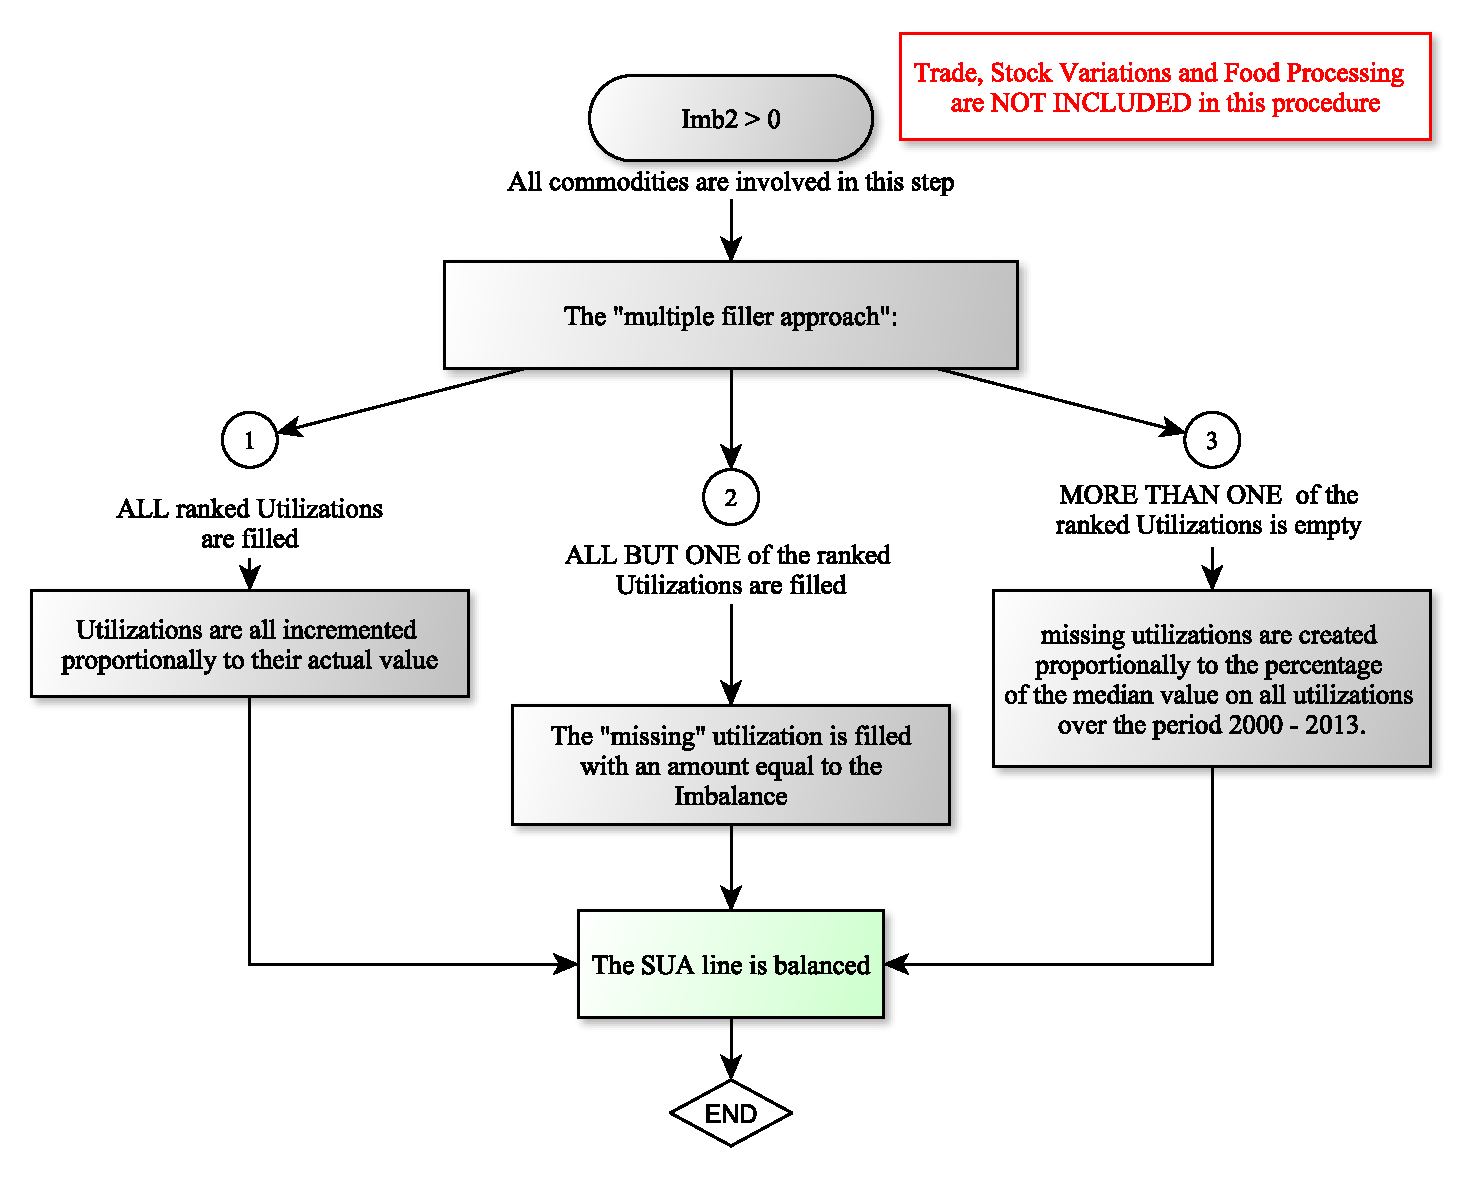
\includegraphics{images/StandBal/07b_PositiveImbalance} 

}

\caption{\label{fig:f5}Workflow of Sua Filling when there is a positive imbalance}\label{fig:f7}
\end{figure}

As reported in the Figure, Three cases may happen:

\begin{enumerate}
\def\labelenumi{\arabic{enumi}.}
\tightlist
\item
  If all the ranked Utilizations are already filled, all of them are
  increased proportionally to their values. \emph{Bran of Wheat} in our
  example, belongs to this case. \emph{Utilization Table} for Bran of
  Wheat is reported in Table 10
\end{enumerate}

\begin{table}

\caption{\label{tab:t9}*Utilization Table* Bran of Wheat - China/Wheat/2014 example}
\centering
\begin{tabular}[t]{c|c|c|c|c}
\hline
AreaM49 & Element & ItemCpc & rank & rankInv\\
\hline
1248 & Fe & 39120.01 & 2 & 2\\
\hline
1248 & Fo & 39120.01 & 1 & 3\\
\hline
1248 & X & 39120.01 & 3 & 1\\
\hline
\end{tabular}
\end{table}

\begin{quote}
According to this table, there are 3 Utilizations that are suppose to be
active for this commodity: \emph{feed}, \emph{food} and \emph{exports}.
\emph{Exports} is excluded from this step, therefore, food and feed
reamain. Both Variables are filled in the SUA line of This Commodity,
therefore, all of them are increased proportionally to their values.
\end{quote}

\begin{enumerate}
\def\labelenumi{\arabic{enumi}.}
\setcounter{enumi}{1}
\item
  If all the ranked Utilizations are already filled but one, the all
  imbalance goes to that commodity. In our Example, this is the case of
  \emph{Gluten Feed and meals} (Table 10).
\item
  Finally, if more that one utilization is empty, the so called
  \textbf{\emph{Inverse Ranking rule}} is activated. This rule assigns
  part of the imbalance to the ranked Utilizations proportionally to the
  ranks. This happens by making use of the inverse rank of all the
  Utilizations that are ``actionable'' and not excluded from the
  procedure. The rule works for any number of ranks and independently
  from the number of Utilizations that have to be excluded.
\end{enumerate}

\begin{quote}
The \emph{Inverse ranking rule} starts from the \emph{Utilization Table}
with the addition of a column containing the \emph{rank weigth \(Wr\)},
as reported in the following table:
\end{quote}

\begin{quote}
\begin{center}
\begin{tabular}{ c|c|c|c } 
\hline
element ($Ut_{h}$) & rank ($r_{h}$) & Inverse rank ($Ir_{h}$) & weight Rank ($Wr_{h}$)\\
\hline
$Ut_{1}$ & $r_{1}$ & $Ir_{1}$  & $Wr_{1}$\\ 
... & ... & ... & ...\\ 
$Ut_{h}$ & $r_{h}$ & $Ir_{h}$  & $Wr_{h}$\\ 
... & ... & ... & ...\\ 
$Ut_{n}$ & $r_{n}$ & $Ir_{n}$  & $Wr_{n}$\\ 
\hline
\end{tabular}
\end{center}
\end{quote}

\begin{quote}
where:
\end{quote}

\begin{quote}
\begin{itemize}
\tightlist
\item
  \(Ut_{h}\) is the generic utilization, with \(h=1,2,...n\)
\item
  \(r_{h}\) is the rank of utilization \(Ut_{h}\), with \(h=1,2,...n\)
\item
  \(hr_{h}\) is the Inverse rank of utilization \(Ut_{h}\), with
  \(h=1,2,...n\) and is equal to:
\end{itemize}
\end{quote}

\begin{quote}
\begin{quote}
\begin{equation}
\label{eq:inverseRankequation}
Ir_{h} = max(r)-r_{h}+1
\end{equation}
\end{quote}
\end{quote}

\begin{quote}
\begin{itemize}
\tightlist
\item
  \(Wr_{h}\) is the rank weight of utilization \(Ut_{h}\) and is equal
  to 0 or 1 depending on the element being, respectively, exluded or not
  from the \emph{Sua Filling} (Table 11).
\end{itemize}
\end{quote}

\begin{table}

\caption{\label{tab:t10}Rank Weight of the elements of FBS}
\centering
\begin{tabular}[t]{c|c}
\hline
Utilizations & Wr\\
\hline
\$X\$ & \$0\$\\
\hline
\$DSt\$ & \$0\$\\
\hline
\$Fo\$ & \$1\$\\
\hline
\$FP\$ & \$0\$\\
\hline
\$Fe\$ & \$1\$\\
\hline
\$Se\$ & \$1\$\\
\hline
\$T\$ & \$1\$\\
\hline
\$IU\$ & \$1\$\\
\hline
\$L\$ & \$1\$\\
\hline
\$ROU\$ & \$0\$\\
\hline
\end{tabular}
\end{table}

\begin{quote}
The value \(V_{h}\) assigned to the Utilizations of each commodity is
calculated as a rank based proportion \(pR_{h}\) of the total \(Imb2\)
according to the following equation:
\end{quote}

\begin{quote}
\begin{equation}
\label{eq:inverseRank}
V_{h} = Imb2 \times pR_{h}
\end{equation}
\end{quote}

\begin{quote}
with \(pR_{h}\) depending on \(\sum \limits_{h=1}^n Wr_{h}\):
\end{quote}

\begin{quote}
\begin{equation}
\label{eq:weightRank}
\begin{cases}
pR_{h} = 0     & \quad \text{when} \quad \sum \limits_{h=1}^n Wr_{h} = 0\\
pR_{h} = \frac{Ir_{h}\times Wr_{h}}{\sum \limits_{i=1}^n\left(Ir_{h}\times Wr_{h}\right)}     & \quad \text{when} \quad \sum \limits_{h=1}^n Wr_{h} > 0 
\end{cases}
\end{equation}
\end{quote}

\begin{quote}
\end{quote}

\begin{quote}
As an example consider the SUA line of \emph{Cocoa Beans} in Madagascar
in 2014 (Table 12) and the \emph{Utilization Table} of the same
country/commodity combination (Table 13)
\end{quote}

\begin{table}

\caption{\label{tab:t11}Sua of Cocoa Beans Madagascar 2014 - before *Sua Filling*}
\centering
\begin{tabular}[t]{c|c|c|c|c|c|c|c|c|c|c|c|c|c}
\hline
itemName & P & I & X & DSt & Fo & FP & Fe & Se & T & IU & L & ROU & Imb2\\
\hline
*Cocoa beans* & 10,865 & 36 & 8,326 & - & - & - & - & - & - & - & 743 & - & ***1,832***\\
\hline
\end{tabular}
\end{table}

\begin{table}

\caption{\label{tab:t12}*Utilization Table* for Cocoa Beans Madagascar}
\centering
\begin{tabular}[t]{c|c|c}
\hline
Ut & relative.median & Wr\\
\hline
FP & 0.00 & 0\\
\hline
Fo & 0.26 & 1\\
\hline
IU & 0.00 & 1\\
\hline
DSt & 0.00 & 0\\
\hline
X & 0.74 & 0\\
\hline
\end{tabular}
\end{table}

\begin{quote}
Besides the excluded elements, there are 2 Utilizations empty:
\emph{food} and \emph{Industrial Use}. The Values \(V_{Fo}\) and
\(V_{IU}\) of these two elements are calculated as follows and the
result shown in Table 14:
\end{quote}

\begin{quote}
\begin{equation}
\begin{aligned}
pR_{Fo} &= \frac{4\times 1}{0 + 0 + 4 + 3 + 0 + 0} = 4/7 = 0.57143 \\
V_{Fo} &= 1,832 \times 0.57143 = 1,047 
\end{aligned}
\end{equation}
\end{quote}

\begin{quote}
\end{quote}

\begin{quote}
\begin{equation}
\begin{aligned}
\label{eq:VIUC}
pR_{IU} &= \frac{3\times 1}{0 + 0 + 4 + 3 + 0 + 0} = 3/7 = 0.42857\\
V_{IU} &= 1,832 \times 0.42857 = 785
\end{aligned}
\end{equation}
\end{quote}

\begin{table}

\caption{\label{tab:t13}Sua line of Cocoa Beans Madagascar 2014 - after *Sua Filling*}
\centering
\begin{tabular}[t]{c|c|c|c|c|c|c|c|c|c|c|c|c|c}
\hline
itemName & P & I & X & DSt & Fo & FP & Fe & Se & T & IU & L & ROU & Imb2\\
\hline
*Cocoa beans* & 10,865 & 36 & 8326 & - & ***1,832*** & - & - & - & - & 0 & 743 & - & ***0***\\
\hline
\end{tabular}
\end{table}

\subsection*{\texorpdfstring{The ``Sua Balanced''
table}{The Sua Balanced table}}\label{the-sua-balanced-table}
\addcontentsline{toc}{subsection}{The ``Sua Balanced'' table}

The table resulting after the \emph{Sua Filling} is called \emph{Sua
Balanced}. For the \emph{China/Wheat/2014} example the \emph{Sua
Balanced} is reported in Table 15.

The red lines are not balanced lines. Indeed, the \emph{Sua Filling}
procedure does not intervene on all the commodities. It leaves
unbalanced all the ``top level'' commodities falling in 2 main
categories:

\begin{enumerate}
\def\labelenumi{\arabic{enumi}.}
\tightlist
\item
  The \emph{Primary commodities}. These are all the crop commodities,
  like cereals, pulses, vegetables, fruits etc, that are often processed
  in other commodities, like the wheat in flour of wheat.
\item
  The \emph{no tree} commodities. These commodities are excluded from
  the list of commodities that are processed into something else, they
  are often mixes of some other crop or commodity and used for specific
  purposes, i.e. \emph{Mixes and dough for the preparation of baker's
  wares} and \emph{Food preparations of Flour, Meal or Malt Extract}
  from our example.
\end{enumerate}

Therefore 3 lines are not balanced in Table 15, belonging to these 2
categories of ``not balanced'' commodities.

\begin{landscape}\begin{table}

\caption{\label{tab:t14}Sua Balanced - China/Wheat/2014 example}
\centering
\resizebox{\linewidth}{!}{
\fontsize{18}{20}\selectfont
\begin{tabular}[t]{r|l|l|l|l|l|l|l|l|l|l|l|l|>{\bfseries\em\raggedright\arraybackslash\leavevmode\color{red}}p{10em}}
\hline
\multicolumn{1}{r}{\textbf{itemName}} & \multicolumn{1}{c}{\textbf{P}} & \multicolumn{1}{c}{\textbf{I}} & \multicolumn{1}{c}{\textbf{X}} & \multicolumn{1}{c}{\textbf{DSt}} & \multicolumn{1}{c}{\textbf{Fo}} & \multicolumn{1}{c}{\textbf{FP}} & \multicolumn{1}{c}{\textbf{Fe}} & \multicolumn{1}{c}{\textbf{Se}} & \multicolumn{1}{c}{\textbf{T}} & \multicolumn{1}{c}{\textbf{IU}} & \multicolumn{1}{c}{\textbf{L}} & \multicolumn{1}{c}{\textbf{ROU}} & \multicolumn{1}{c}{\textbf{Imb2}}\\
\hline
Wheat & 126,208,400 & 2,971,249 & 957 & 1,079,280 &  & 90,384,615 & 28,106,487 & 84,119,970 &  & 2,875,293 & 2,613,046 & - & 0\\
\hline
Wheat and meslin flo & 70,500,000 & 33,055 & 188,674 &  & 68,372,646 & 1,958,146 &  &  & -17,621 &  &  & - & 0\\
\hline
Mixes and doughs for & 31,575 & 6,497 & 38,072 &  & 0 &  & 0 &  & 0 &  &  & - & 0\\
\hline
Other Fructose and S & 158,665 & 3,659 & 162,324 &  & 0 &  &  &  & 0 &  &  & - & 0\\
\hline
Starch of Wheat & 314,020 & 11,035 & 40,311 &  &  & 158,664 & 120,537 &  &  & 5,543 &  & - & 0\\
\hline
Wheat Gluten & 381,076 & 877 & 117,373 &  &  & 0 & 0 &  &  &  &  & - & 0\\
\hline
Communion wafers & 13,263 & 8,796 & 5,822 &  & 16,241 &  &  &  & -4 &  &  & - & 0\\
\hline
Uncooked pasta & 1,415,692 & 12,520 & 22,550 &  & 1,406,024 &  &  &  & -363 &  &  & - & 0\\
\hline
Food Preparations of &  & 69,686 & 21,977 &  & 47,721 &  &  &  & -12 &  &  & - & 0\\
\hline
Bran of Wheat & 21,414,279 & 156,359 & 2,200 &  & 16,689,929 &  & 4,882,810 &  & -4,301 &  &  & - & 0\\
\hline
Gluten Feed and Meal & 793,740 & 160,230 & 529,333 &  &  &  & 424,637 &  &  &  &  & - & 0\\
\hline
bread & 15,485 & 2,897 & 4,210 &  & 14,175 &  &  &  & -3 &  &  & - & 0\\
\hline
pastry & 193,950 & 89,593 & 117,630 &  & 165,957 &  &  &  & -42.75 &  &  & - & 0\\
\hline
\multicolumn{14}{l}{\textsuperscript{a} \makecell[l]{P=Production, I=Import, X=Export, DSt=Delta Stock, Fo=Food Availability, FP=FoodProcessing,\\ Fe=Feed, Se=Seed, T=Tourism Consumption, IU=IndustrialUse, L=Loss, ROU=Residual and other uses}}\\
\end{tabular}}
\end{table}
\end{landscape}

\emph{Zero-level} commodities are excluded form the filling because the
standardization will affect the figures of the primary commodities, this
opening the need for a final \emph{balancing} procedure. In order not to
intervene twice on these commodities, it has been decide to keep as
smaller as possible the number correction, so to reduce error.

\subsection*{Nutritive Values and DES
calculation}\label{nutritive-values-and-des-calculation}
\addcontentsline{toc}{subsection}{Nutritive Values and DES calculation}

After the \emph{sua Balanced} table has been produced,
\textbf{\emph{Nutritive values}} are calculated (\emph{Calories},
\emph{Proteins} and \emph{Fats}), based on the Food availability
produced during the \emph{Sua Filling}. These Variables are calculated
for each Food Product of the SUA, based on official Nutritive Factors
stored in the SWS. Values of Nutritive elements are stored in the system
as:

\begin{itemize}
\tightlist
\item
  \(g/100g\), for Proteins and Fats
\item
  \(Kcal/100g\) for Calories.
\end{itemize}

As a consequence, the amount of Nutritive Elements for the number of
Tonnes of Food is given by

\begin{equation}
\label{eq:Nutritive}
\text{Nutritive value} = \text{Nutritive factor} \times \text{Food availability (tonnes)} \times 10,000
\end{equation}

In particular, after all Nutritive Values are calculated, only DES is
reported for FBS's purposes, DES being given by:

\begin{equation}
\label{eq:des}
 DES_{ijt} = \cfrac{\cfrac{Kcal_{ijt}}{Population_{jt}}}{365}
\end{equation}

where the \(i\) index runs over all countries, the \(j\) index over all
commodities, and \(t\) over years.

DES for the food commodities in the \emph{China/Wheat/2014} example are
reported in Table 16

\begin{table}

\caption{\label{tab:t19}Sua Unbalanced DES - China/Wheat/2014 example}
\centering
\begin{tabular}[t]{c|c|c}
\hline
itemName & Fo & DES\\
\hline
Wheat & - & -\\
\hline
Wheat and meslin flo & 68,372,646 & 478.38\\
\hline
Mixes and doughs for & 0 & 0\\
\hline
Other Fructose and S & 0 & 0\\
\hline
Starch of Wheat & - & -\\
\hline
Wheat Gluten & - & -\\
\hline
Communion wafers, em & 16,239.38 & 0.1405\\
\hline
Uncooked pasta, not & 1,406,024 & 10.1699\\
\hline
Food Preparations of & 47,708.53 & 0.3545\\
\hline
Bran of Wheat & 16,689,929 & 70.0635\\
\hline
Gluten Feed and Meal & - & -\\
\hline
bread & 14,174.09 & 0.0696\\
\hline
pastry & 165,957 & 1.2069\\
\hline
\end{tabular}
\end{table}

Figure \ref{fig:f8} Represents the steps following the \emph{Sua
Filling}:

\begin{figure}[H]

{\centering 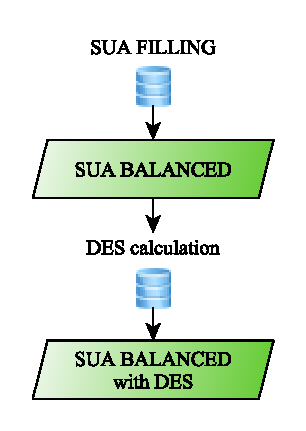
\includegraphics{images/StandBal/08_SuaBalanced} 

}

\caption{\label{fig:f8}Sua Balanced and the calculation of DES}\label{fig:f8}
\end{figure}

\section{Standardization}\label{standardization}

The \emph{Standardization} is the process of transforming all the
processed commodities in terms of their primary (or
\emph{proxy-primary}) commodities and to add up all the calories of the
food commodities. This produces all the existing food availability of a
country expressed in terms of the main commodities. Aggregation of data
from a detailed product classification to a more comprehensive one is
common practice for two reasons. The first reason is to reduce the
amount of data, and the number of commodities involved, to a level and
size more suited for analytic purposes. The second reason is, that by
cancelling out the intermediate production of derived products against
the input use of primary products, a clearer view emerges of the
domestic availability of a product and its final uses.

\begin {table}[H]
\begin{center}
\caption {Generic SUA for Standardization for country j and time t}

\begin{tabular}{lllllllllllll}
& & & & & \\
 \hline
Item & $el^{*}_{1}$ & ... & $el^{*}_{h}$ & ...& $el^{*}_{n}$ & $Kcal$\\ 
 \hline
$parent_{p}$ & $V_{p1}$ & ...& $V_{ph}$ & ...& $V_{pn}$ & $Kcal_{p}$\\ 
$child_{1}$ & $V_{11}$ & ... & $V_{1h}$ & ...& $V_{1n}$ & $Kcal_{1}$\\ 
... & ... & ... & ... & ... & ... & ... & \\ 
$child_{c}$ & $V_{c1}$ & ... & $V_{ch}$ & ...& $V_{cn}$ & $Kcal_{c}$\\ 
... & ... & ... & ... & ... & ... & ... & \\ 
$child_{C}$ & $V_{C1}$ & ... & $V_{Ch}$ & ...& $V_{Cn}$ & $Kcal_{C}$\\ 
 \hline
\end{tabular}
\end{center}
\end {table}

The standardization starts from the SUA table reported, in its generic
form, in Table 17,where country and time indexes are omitted and where:

\begin{itemize}
\tightlist
\item
  \(c = 1,2,3...C\) are the \(C\) children \(c\) of parent \(p\),
\item
  \(V_{ch}\) is Value of element \(h\) for child \(c\),
\item
  \(V_{ph}\) is Value of element \(h\) for parent \(p\),
\item
  \(el^{*}_{h}\) is the generic Element of the generic child \(c\) of
  Parent \(p\) in the range of elements involved in the Standardization.
  Indeed, \(P\) and \(FP\) are excluded from this step of the process:
\end{itemize}

\begin{quote}
\(el^{*} \in E^{*} = \{I,X,\Delta St, ,Fo,Fe,Lo,Se,IU,T,ROU\}\)
\end{quote}

\begin{itemize}
\tightlist
\item
  \(Kcal\) is the amount of Calories associated with the commodity. This
  is positive only if the commodity is a food commodity.
\end{itemize}

Standardize a SUA is the process of:

\begin{enumerate}
\def\labelenumi{\alph{enumi}.}
\tightlist
\item
  expressing the vales of all elements \(V_{ch}\) of the children of a
  parent commodity, in terms of their parent commodity,
\item
  Adding up all the calories of the food commodities and calculate DES.
\end{enumerate}

Elements are transformed in their parent commodity following the
equation:

\begin{equation}
\begin{cases}
\label{eq:Food Processing}
 V_{ph} = \sum \limits_{c=1}^C\biggl(\frac{V_{ch}}{eR_{p\to c}}\biggr)\times s^{2}_{cp}\times w_{c}\\
  \\
 DES_{p} =  \cfrac{\cfrac{Kcal_{p} + \sum \limits_{c=1}^C Kcal_{c}}{Population}}{365}
\end{cases}
\end{equation}

\begin{quote}
where, for country \(j\) and time \(t\):
\end{quote}

\begin{itemize}
\tightlist
\item
  \(c = 1,2,3...C\) are the \(C\) children \(c\) of parent \(p\),
\item
  \(eR_{p\to c}\) is the \emph{extraction Rate} from parent \(p\) to
  child \(c\),
\item
  \(w_{c}\) is the \emph{weight} of child \(c\),
\item
  \(Kcal_{p}\) are the Kcal of the parent commodity (if is a food
  commodity),
\item
  \(Kcal_{c}\) are the Kcal of the child commodities,
\item
  \(s^{2}_{cp}\) is the \emph{share} of child \(c\) from parent \(p\)
  and is based on a different availability from the previous one:
\end{itemize}

\begin{equation}
\label{eq:shares}
s^{2}_{cp} = \cfrac{availability2_{p(c)}}{\sum \limits_{p=1}^A{availability2_{p(c)}}}
\end{equation}

\begin{quote}
where \(availability2_{p(c)}\) is the availability of each parent \(p\)
of child \(c\) expressed in terms of \(c\) (as say in \emph{child
equivalent}). Is is enumerated as \(2\) because is different from the
one previously defined. Indeed, here The availability of each parent is
the amount of that commodity available to be processed, i.e.~the Food
processing, expressed in terms of child, therefore:
\end{quote}

\begin{quote}
\begin{quote}
\begin{equation}
\label{eq:availability2}
availability2_{p(c)} = FP_{p}\times eR_{p\to c}
\end{equation}
\end{quote}
\end{quote}

\begin{table}

\caption{\label{tab:t17}Availabilities and shares of parent/child for Standardization}
\centering
\begin{tabular}[t]{c|c|c|c|c|c}
\hline
Child & Parent & extractionRate & availability & share & weight\\
\hline
Wheat and meslin flo & Wheat & 0.78 & 70,500,000 & 1.00 & 1\\
\hline
Bran of Wheat & Wheat & 0.22 & 19,884,615 & 1.00 & 0\\
\hline
Uncooked pasta, not & Wheat & 0.78 & 72,458,146 & 1.00 & 1\\
\hline
Germ of Wheat & Wheat & 0.02 & 1,920,221 & 1.00 & 0\\
\hline
bread & Wheat & 0.78 & 72,458,146 & 1.00 & 1\\
\hline
Bulgur & Wheat & 0.95 & 85,865,385 & 1.00 & 1\\
\hline
pastry & Wheat & 0.78 & 72,458,146 & 1.00 & 1\\
\hline
Starch of Wheat & Wheat & 0.58 & 54,343,610 & 1.00 & 1\\
\hline
Wheat Gluten & Wheat & 0.06 & 5,796,652 & 1.00 & 0\\
\hline
Communion wafers, em & Wheat & 0.78 & 72,458,146 & 1.00 & 1\\
\hline
Other Fructose and S & Wheat & 0.58 & 54,502,275 & 1.00 & 1\\
\hline
Gluten Feed and Meal & Wheat & 0.06 & 5,796,652 & 0.76 & 0\\
\hline
Gluten Feed and Meal & Maize (corn) & 0.09 & 1,803,440 & 0.24 & 0\\
\hline
\end{tabular}
\end{table}

Table 18 shows the values of \(availability2\), \(eR\) and \emph{shares}
and \emph{weights} of the \emph{China/Wheat/2014} example.

Comparing this table with Table 15:

\begin{equation}
\label{eq:avExample1}
availability2_{wheat(flour)} = 90,384,615\times 0,78 = 70,500,000
\end{equation}

\begin{equation}
\label{eq:avExample2}
availability2_{wheat(bran)} = 90,384,615\times 0,22 = 19,884,615
\end{equation}

Moreover:

\begin{equation}
\label{eq:shareEx1}
s^{2}_{Gluten,wheat} = \frac{5,796,652}{5,796,652 + 1,803,440} = 0.76
\end{equation}\begin{equation}
\label{eq:shareEx1}
s^{2}_{Gluten,Maize} = \frac{1,803,440}{5,796,652 + 1,803,440} = 0.24
\end{equation}

By applying equations \ref{eq:Food Processing} to \ref{eq:availability2}
to Table 15, Table 20 is obtained, which contains the so
\emph{Standardized} Table, while the DES for the \emph{Sua Standardized}
of Table 20 is reported in Table 19.

\begin{table}

\caption{\label{tab:t20}DES of *Sua Standardized* - China/Wheat/2014 example}
\centering
\begin{tabular}[t]{c|c}
\hline
itemName & DES\\
\hline
Wheat & 560.0300\\
\hline
Mixes and doughs for & 0.0000\\
\hline
Food Preparations of & 0.3545\\
\hline
\end{tabular}
\end{table}

Notice that \emph{Production} remains untouched from the Standardization
process and \emph{ROU} are still untouched.

\subsection*{\texorpdfstring{The ``Fbs Standardized''
table}{The Fbs Standardized table}}\label{the-fbs-standardized-table}
\addcontentsline{toc}{subsection}{The ``Fbs Standardized'' table}

The standardized table is called \emph{Fbs Standardized} and is composed
of more than 1 line, because, besides the primary commodity there are 2
more typologies of commodities, both :

\begin{itemize}
\tightlist
\item
  \emph{No-tree} commodities, that are also \emph{``zero-level''}
  commodities, appear here as they were in the previous step. Indeed, as
  these are not processed, the standardization does not change any of
  the element's values.
\item
  \emph{Proxy-primary} commodities. The Child commodities defined as
  \emph{proxy-primary} are cut from their trees immediately before the
  standardization begins. They are treated as primary commodities and
  appear here together with the primaries.
\end{itemize}

Table 20 and Table 23

\begin{landscape}\begin{table}

\caption{\label{tab:t18}Sua Standardized}
\centering
\resizebox{\linewidth}{!}{
\fontsize{18}{20}\selectfont
\begin{tabular}[t]{>{\raggedleft\arraybackslash}p{10em}|>{\raggedright\arraybackslash\leavevmode\color{black}}p{6em}|>{\raggedright\arraybackslash\leavevmode\color{black}}p{6em}|>{\raggedright\arraybackslash\leavevmode\color{black}}p{6em}|>{\raggedright\arraybackslash\leavevmode\color{black}}p{6em}|>{\raggedright\arraybackslash\leavevmode\color{black}}p{6em}|>{\raggedright\arraybackslash\leavevmode\color{black}}p{6em}|>{\raggedright\arraybackslash\leavevmode\color{black}}p{6em}|>{\raggedright\arraybackslash\leavevmode\color{black}}p{6em}|>{\raggedright\arraybackslash\leavevmode\color{black}}p{6em}|>{\raggedright\arraybackslash\leavevmode\color{black}}p{6em}|>{\raggedright\arraybackslash\leavevmode\color{black}}p{6em}|>{\raggedright\arraybackslash\leavevmode\color{black}}p{6em}}
\hline
\multicolumn{1}{r}{\textbf{itemName}} & \multicolumn{1}{c}{\textbf{P}} & \multicolumn{1}{c}{\textbf{I}} & \multicolumn{1}{c}{\textbf{X}} & \multicolumn{1}{c}{\textbf{DSt}} & \multicolumn{1}{c}{\textbf{Fo}} & \multicolumn{1}{c}{\textbf{FP}} & \multicolumn{1}{c}{\textbf{Fe}} & \multicolumn{1}{c}{\textbf{Se}} & \multicolumn{1}{c}{\textbf{T}} & \multicolumn{1}{c}{\textbf{IU}} & \multicolumn{1}{c}{\textbf{L}} & \multicolumn{1}{c}{\textbf{ROU}}\\
\hline
Wheat & 126,208,400 & **3,184,654** & **781,808** & 1,120,565 & **89,711,591** & **0** & **29,387,664** & 4,277,567 & **-22,766.5** & **2,994,755** & 2,713,000 & -\\
\hline
Mixes and doughs for & - & 6,496.91 & 38,071.88 & 0 & 0 & 0 & 0 & 0 & 0 & 0 & 0 & -\\
\hline
Food Preparations of & - & 69,685.96 & 21,977.43 & 0 & 47,708.53 & 0 & 0 & 0 & -12.2958 & 0 & 0 & -\\
\hline
\multicolumn{13}{l}{\textsuperscript{a} P=Production, I=Import, X=Export, DSt=Delta Stock, Fo=Food Availability, FP=FoodProcessing, Fe=Feed, Se=Seed, T=Tourism Consumption, IU=IndustrialUse, L=Loss, ROU=Residual and other uses}\\
\multicolumn{13}{l}{\textsuperscript{b} Starred figures are those that have changed from the previous table}\\
\end{tabular}}
\end{table}
\end{landscape}

\section{The FBS Balancing}\label{the-fbs-balancing}

The balancing of Standardized Sua in the new framework is based on the
idea that, at this step of the overall process, a \emph{little}
imbalance has been cumulated, due to the errors of each variable. The
FBS equation can be thought as being composed by each variable and its
measurement error (\(ME\)).

\begin{multline}
\label{eq:balance_b}
    P + ME_{P} + I + ME_{I} - \Delta St + ME_{\Delta St} = X + ME_{X} + Fo +ME_{Fo} + Fe + ME_{Fe} + Lo + ME_{Lo} \\
    + Se + ME_{Se} + IU + ME_{IU} + T + ME_{T} + ROU + ME_{ROU}
\end{multline}

Because is not possible to know the \(ME\) a-priori, an approach is
based that computes adjustment values for each variable proportionally
to some \emph{a-priori allowed percentages of variation}

Therefore, equation \ref{eq:balance1} can be rewritten, in its balanced
form, as:

\begin{equation}
\label{eq:balance3}
P^*_{ijt} + I^*_{ijt} - X^*_{ijt} - \Delta St^*_{ijt} = FP^*_{ijt} + Fo^*_{ijt} + Fe^*_{ijt} + Lo^*_{ijt} + Se^*_{ijt} + IU^*_{ijt} + T^*_{ijt}  + ROU^*_{ijt}
\end{equation}

where (dropping the indices for brevity):

\begin{itemize}
\tightlist
\item
  \(P^* = P \mp adj_{P}\)
\item
  \(I^* = I \mp adj_{I}\)
\item
  \(X^* = X \pm adj_{X}\)
\item
  \(\Delta St^* = \Delta St \pm adj_{\Delta St}\)
\item
  \(FP^* = FP \pm adj_{FP}\)
\item
  \(Fo^* = Fo \pm adj_{Fo}\)
\item
  \(Fe^* = Fe \pm adj_{Fe}\)
\item
  \(Lo^* = Lo \pm adj_{Lo}\)
\item
  \(Se^* = Se \pm adj_{Se}\)
\item
  \(IU^* = IU \pm adj_{IU}\)
\item
  \(T^* = T \pm adj_{T}\)
\end{itemize}

and where each \emph{adjustment (\(adj_{el \in E}\))} is a balancing
adjustment calculated starting from \emph{a-priori allowed percentages
of variation} for each element
\(el \in E = \{P,I,X,\Delta St, FP,Fo,Fe,Lo,Se,IU,T,ROU\}\).

The process is a two-step process. It start with the definition of the
\emph{allowed percentages of variation} \emph{(\(varP_{el \in E}\))} for
each element as reported in the following Table:

\begin{table}

\caption{\label{tab:t21}Measurement Errors percentages}
\centering
\begin{tabular}[t]{c|c}
\hline
\$el\$ & \$varP\_\{el\}\$\\
\hline
\$P\$ & \$0.1\textbackslash{}\%\$\\
\hline
\$I\$ & \$1\textbackslash{}\%\$\\
\hline
\$X\$ & \$1\textbackslash{}\%\$\\
\hline
\$DSt\$ & \$25\textbackslash{}\%\$\\
\hline
\$Fo\$ & \$5\textbackslash{}\%\$\\
\hline
\$FP\$ & \$25\textbackslash{}\%\$\\
\hline
\$Fe\$ & \$25\textbackslash{}\%\$\\
\hline
\$Se\$ & \$25\textbackslash{}\%\$\\
\hline
\$T\$ & \$25\textbackslash{}\%\$\\
\hline
\$IU\$ & \$25\textbackslash{}\%\$\\
\hline
\$L\$ & \$25\textbackslash{}\%\$\\
\hline
\$ROU\$ & \$0\$\\
\hline
\end{tabular}
\end{table}

\(ROU\) is not included int his table because ROU is created in this
step in a slightly different way.

Indeed, the \emph{final balancing} happens according to the Residual and
Other Uses is set equal to the Imbalance steps (figure \ref{fig:f10}:

\begin{figure}[H]

{\centering 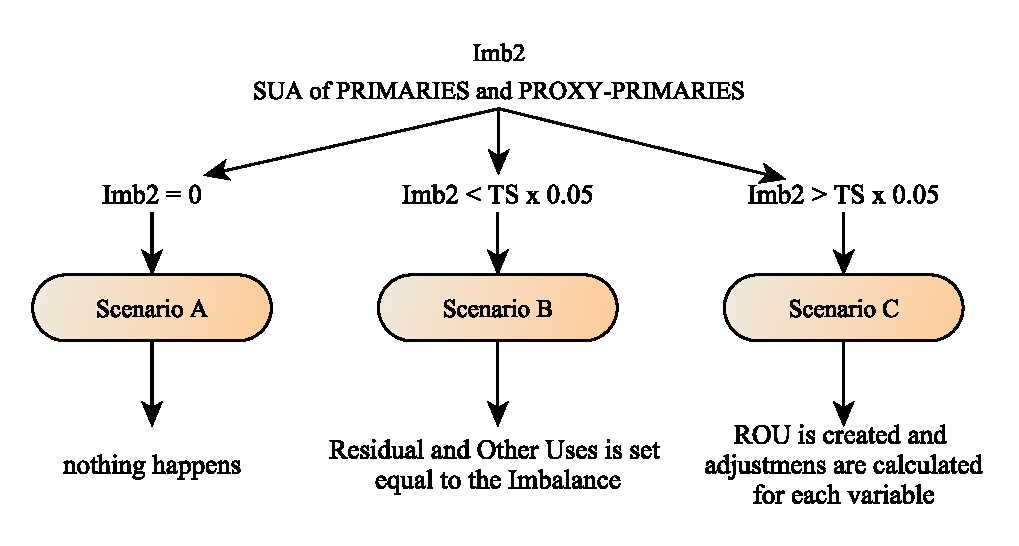
\includegraphics[width=1\linewidth]{images/StandBal/11_ScenariosFinalBal} 

}

\caption{\label{fig:f10}Scenarios of the final balancing}\label{fig:f10}
\end{figure}

\textbf{1.} If \(Imb2 > 0\):

\begin{itemize}
\item
  \textbf{1.a} If \(Imb2 < TS \times 0.05\):

  \begin{quote}
  Residual and Other Uses is set equal to the Imbalance:
  \end{quote}

  \begin{quote}
  \(ROU = Imb2\)
  \end{quote}

  \begin{quote}
  and the equation is balanced.
  \end{quote}
\item
  \textbf{1.b} If \(Imb2 > TS \times 0.05\):

  \begin{itemize}
  \tightlist
  \item
    \(ROU^* = TS \times 0.05\)
  \item
    \(Imb2 = Imb2 - ROU^*\)
  \item
    The \emph{\(adj_{el \in E}\)}s are given by:
  \end{itemize}
\end{itemize}

\begin{quote}
\begin{quote}
\begin{equation}
\label{eq:badj1}
adj_{el \in E} = Imb2 \times V_{el} \times p_{adj_{el}}
\end{equation}
\end{quote}
\end{quote}

\begin{quote}
\begin{quote}
with
\end{quote}
\end{quote}

\begin{quote}
\begin{quote}
\begin{equation}
\label{eq:badj2}
p_{adj_{el}} =\cfrac{varP_{el}}{\sum \limits_{el \in E} (V_{el} \times varP_{el \in E})}
\end{equation}
\end{quote}
\end{quote}

\begin{quote}
\begin{quote}
and
\end{quote}
\end{quote}

\begin{quote}
\begin{quote}
\begin{equation}
\label{eq:badj3}
\sum \limits_{el \in E} p_{adj_{el}} = 1
\end{equation}
\end{quote}
\end{quote}

\begin{quote}
\begin{quote}
adjustments here are considered with Positive sign for utilization and
negative for Supply.
\end{quote}
\end{quote}

\textbf{2.} If Imbalance is Negative: \(Imb2 < 0\)

\begin{quote}
\emph{ROU} is not activated and the other elements are balanced
accordingly to equations \ref{eq:badj1} to \ref{eq:badj3}, with the
opposite sign.
\end{quote}

\subsection*{Nutritive Values updates}\label{nutritive-values-updates}
\addcontentsline{toc}{subsection}{Nutritive Values updates}

After the balancing happens, the value of Food availability might have
changed, therefore, the Nutritive values have to be adjusted
accordingly. The \emph{Balanced Nutritive values} are obtained through a
proportion. For the \emph{DES}, this proportion is given by:

\(V^*_{Fo} : V_{Fo} = DES^* : DES \rightarrow DES^* = DES \times \cfrac{V^*_{Fo}}{V_{Fo}}\)

Table 22 reports all the steps of the final balancing in the
China/Wheat/2014 example for \emph{Wheat}, including the final
adjustment of the DES.

\begin{table}

\caption{\label{tab:t22}Final Balancing - China/Wheat/2014 - Wheat}
\centering
\begin{tabular}[t]{r|l|l|l|l|l|l|l|l}
\hline
\textbackslash{}boldmath\$el\$ & \textbackslash{}boldmath\$V\_\{el \textbackslash{}in E\}\$ & \textbackslash{}boldmath\$varP\$ & \textbackslash{}boldmath\$V\_\{el\} \textbackslash{}times varP\$ & \textbackslash{}boldmath\$p\_\{adj\_\{el\}\}\$ & \textbackslash{}boldmath\$adj\_\{el \textbackslash{}in E\}\$ & \textbackslash{}boldmath\$V\textasciicircum{}*\_\{el \textbackslash{}in E\}\$ & \textbackslash{}boldmath\$DES\$ & \textbackslash{}boldmath\$DES\textasciicircum{}*\$\\
\hline
\$P\$ & 126,208,400 & 0.001 & 126,208 & 0.01 & 13,426 & 126,221,826 & - & -\\
\hline
\$I\$ & 3,184,654 & 0.01 & 31,847 & 0 & 3,388 & 3,188,042 & - & -\\
\hline
\$X\$ & 781,808 & 0.01 & 7,818 & 0 & -832 & 780,976 & - & -\\
\hline
\$\textbackslash{}Delta St\$ & 1,120,565 & 0.25 & 280,141 & 0.02 & -29,801 & 1,090,764 & - & -\\
\hline
\$Fo\$ & 89,711,591 & 0.05 & 4,485,580 & 0.3 & -477,172 & 89,234,419 & 560.03 & ***557.05***\\
\hline
\$FP\$ & 0 & 0.01 & 0 & 0 & 0 & 0 & - & -\\
\hline
\$Fe\$ & 29,387,664 & 0.25 & 7,346,916 & 0.5 & -781,559 & 28,606,105 & - & -\\
\hline
\$Se\$ & 4,277,567 & 0.25 & 1,069,392 & 0.07 & -113,761 & 4,163,806 & - & -\\
\hline
\$T\$ & -22,766.50 & 0.25 & -5,692 & 0 & 605 & -22,161 & - & -\\
\hline
\$IU\$ & 2,994,755 & 0.25 & 748,689 & 0.05 & -79,645 & 2,915,110 & - & -\\
\hline
\$L\$ & 2,713,000 & 0.25 & 678,250 & 0.05 & -72,152 & 2,640,848 & - & -\\
\hline
\$ROU\$ & - & - & - & - & - & - & - & -\\
\hline
\textbackslash{}boldmath\$Imb2\$ & **-1,571,130** & - & - & - & - & ***0*** & - & -\\
\hline
\textbackslash{}boldmath\$\textbackslash{}sum \textbackslash{}limits\_\{el \textbackslash{}in E\}\$ &  &  & **14,769,149** & - & - & - & - & -\\
\hline
\end{tabular}
\end{table}

The balancing of the commodity \emph{Food Preparations of} is reported
in Table 23. In this case, the imbalance is positive and absorbed by the
element \emph{ROU}.

\newpage

\begin{table}

\caption{\label{tab:t24}Final Balancing - China/Wheat/2014 - Food Preparations}
\centering
\begin{tabular}[t]{r|l|l|l|l}
\hline
\textbackslash{}boldmath\$el\$ & \textbackslash{}boldmath\$V\_\{el \textbackslash{}in E\}\$ & \textbackslash{}boldmath\$V\textasciicircum{}*\_\{el \textbackslash{}in E\}\$ & \textbackslash{}boldmath\$DES\$ & \textbackslash{}boldmath\$DES\textasciicircum{}*\$\\
\hline
\$P\$ &  &  & - & -\\
\hline
\$I\$ & 69,685.96 & 69,685.96 & - & -\\
\hline
\$X\$ & 21,977.43 & 21,977.43 & - & -\\
\hline
\$\textbackslash{}Delta St\$ & 0 & 0 & - & -\\
\hline
\$Fo\$ & 47,708.53 & 47,708.53 & 0.3545 & 0.3545\\
\hline
\$FP\$ & 0 & 0 & - & -\\
\hline
\$Fe\$ & 0 & 0 & - & -\\
\hline
\$Se\$ & 0 & 0 & - & -\\
\hline
\$T\$ & -12.2958 & -12.2958 & - & -\\
\hline
\$IU\$ & 0 & 0 & - & -\\
\hline
\$L\$ & 0 & 0 & - & -\\
\hline
\$ROU\$ & - & 12 & - & -\\
\hline
\textbackslash{}boldmath\$Imb2\$ & **12** & ***0*** & - & -\\
\hline
\textbackslash{}boldmath\$TS\$ & **69,685.96** & - & - & -\\
\hline
\textbackslash{}boldmath\$TS \textbackslash{}times 0.05\$ & **3,484.298** &  &  & \\
\hline
\textbackslash{}boldmath\$|Imb2| < TS \textbackslash{}times 0.05\$ & **TRUE** &  &  & \\
\hline
\end{tabular}
\end{table}

\section{Final aggregation: FBS items and FBS
aggregates}\label{final-aggregation-fbs-items-and-fbs-aggregates}

The Food Balance Sheets have to be expressed in \emph{FBS} items.The
conversion from CPC to FBS is a simple aggregation based on an
aggregation table, called \textbf{\emph{Fbs Tree}}, an extract of which
is reported in Table 24.

After the Balancing happens, the CPC commodities are aggregated on the
basis of the classifications of FBS commodities reported in the table. 3
different level of aggregations are performed:

\begin{enumerate}
\def\labelenumi{\arabic{enumi}.}
\tightlist
\item
  at FBS item level,
\item
  At FBS group level
\item
  at FBS family level
\item
  at the Total (By country) FBS Level.
\end{enumerate}

Table 25 reports these aggregations for the China/Wheat/2014 example,
including the DES.

\begin{table}[ht]
\caption {Fbs Tree [extraction of the main table]}
\centering
\resizebox{\columnwidth}{!}{
\begin{tabular}{l|l|l|l|l}
\toprule
\multicolumn{4}{c|}{\bf{FBS}} & \multicolumn{1}{c}{\bf{SUA}}\\ 
\midrule
\bf{TOTAL} & \bf{FAMILY} & \bf{GROUP} & \bf{ITEM} & \bf{P-P \& PROC*} \\ 
\midrule
\multirow{47}{*}{2901 GRAND TOTAL} & \multirow{37}{*}{2903  VEGETALE PRODUCTS}  & \multirow{22}{*}{2905 CEREALS (EXCLUDING BEER)} & \multirow{14}{*}{2511 WHEAT \& PRODUCTS}  & WHEAT \\ 
&  &  &  & FLOUR WHEAT \\ 
&  &  &  & BRAN WHEAT  \\ 
&  &  &  & MACARONI \\ 
&  &  &  & GERM WHEAT  \\ 
&  &  &  & BREAD \\ 
&  &  &  & BULGUR \\ 
&  &  &  & PASTRY \\ 
&  &  &  & WHEAT,STARCH \\ 
&  &  &  & WHEAT GLUTEN  \\ 
&  &  &  & BREAKF CERLS \\ 
&  &  &  & WAFERS \\ 
&  &  &  & MIXES AND DO  \\ 
&  &  &  & FOOD PREP.FL  \\ 
\cline{4-5}
&  &  &  \multirow{7}{*}{2514 MAIZE \& PRODUCTS}  & MAIZE \\ 
&  &  &  & GERM MAIZE  \\ 
&  &  &  & FLOUR MAIZE \\ 
&  &  &  & BRAN MAIZE  \\ 
&  &  &  & MAIZE GLUTEN  \\ 
&  &  &  & STARCH MAIZE \\ 
&  &  &  & GLUT FEED\& ME \\ 
&  & … & … & … \\
\cline{3-5}
&  & \multirow{11}{*}{2909 SWEETENERS} & \multirow{11}{*}{2543 SWEETENERS, OTHER \& PROD} & FRUCTOSE CHE \\ 
&  &  &  & MALTOSE CHEM \\ 
&  &  &  & MAPLE SUGAR \\ 
&  &  &  & SUGAR CROPS \\ 
&  &  &  & MOLASSES (calories \\ 
&  &  &  & OTHER FRUCTO \\ 
&  &  &  & SUGAR NES \\ 
&  &  &  & GLUC. DEXTR. \\ 
&  &  &  & LACTOSE \\ 
&  &  &  & ISOGLUCOSE \\ 
&  &  &   & BEV NON-ALC \\ 
&  & … & … & … \\
\cline{3-5}
&  & \multirow{2}{*}{2914 VEGETABLE OILS} & 2571 SOYABEAN, OIL & OIL SOYABEAN \\ 
&  &  & 2572 GROUNDNUT, OIL 2 & OIL GROUNDNT \\ 
& … & … & … & … \\
\cline{2-5}
& \multirow{10}{*}{2941  ANIMAL PRODUCTS}  & \multirow{10}{*}{2943 MEAT (SLAUGHTERED)}  & \multirow{10}{*}{2731 MEAT \& PRODUCTS BOVINE}  & BEEF VEAL \\ 
&  &   &  & BEEF BONLESS \\ 
&  &  &  & BEEF DSS \\ 
&  &  &  & MEAT EXTRACT \\ 
&  &  &  & SAUSAGE BEEF \\ 
&  &  &  & BEEF PREP \\ 
&  &  &  & BEEF CANNED \\ 
&  &  &  & HOMOGENIZED \\ 
&  &  &  & BUFFALO MEAT \\ 
& … & … & … & … \\
\bottomrule
\\
\multicolumn{5}{c|}{* P-P \& PROC stands for "Proxy-primaries and Processed commodities"}
\end{tabular}
}
\end{table}

\begin{landscape}\begin{table}

\caption{\label{tab:t25}FBS Final Aggregations - China/Wheat/2014}
\centering
\resizebox{\linewidth}{!}{
\fontsize{18}{20}\selectfont
\begin{tabular}[t]{>{\raggedleft\arraybackslash}p{10em}|>{\raggedright\arraybackslash\leavevmode\color{black}}p{6em}|>{\raggedright\arraybackslash\leavevmode\color{black}}p{6em}|>{\raggedright\arraybackslash\leavevmode\color{black}}p{6em}|>{\raggedright\arraybackslash\leavevmode\color{black}}p{6em}|>{\raggedright\arraybackslash\leavevmode\color{black}}p{6em}|>{\raggedright\arraybackslash\leavevmode\color{black}}p{6em}|>{\raggedright\arraybackslash\leavevmode\color{black}}p{6em}|>{\raggedright\arraybackslash\leavevmode\color{black}}p{6em}|>{\raggedright\arraybackslash\leavevmode\color{black}}p{6em}|>{\raggedright\arraybackslash\leavevmode\color{black}}p{6em}|>{\raggedright\arraybackslash\leavevmode\color{black}}p{6em}|>{\raggedright\arraybackslash\leavevmode\color{black}}p{6em}|>{\raggedright\arraybackslash\leavevmode\color{black}}p{6em}}
\hline
\multicolumn{1}{r}{\textbf{commodity}} & \multicolumn{1}{c}{\textbf{P}} & \multicolumn{1}{c}{\textbf{I}} & \multicolumn{1}{c}{\textbf{X}} & \multicolumn{1}{c}{\textbf{DSt}} & \multicolumn{1}{c}{\textbf{Fo}} & \multicolumn{1}{c}{\textbf{FP}} & \multicolumn{1}{c}{\textbf{Fe}} & \multicolumn{1}{c}{\textbf{Se}} & \multicolumn{1}{c}{\textbf{T}} & \multicolumn{1}{c}{\textbf{IU}} & \multicolumn{1}{c}{\textbf{L}} & \multicolumn{1}{c}{\textbf{ROU}} & \multicolumn{1}{c}{\textbf{DES}}\\
\hline
WHEAT \& PROD. & 126,221,780 & 3,272,192 & 813,228 & 1,090,866 & 89,283,771 & 0 & 28,608,797 & 4,164,198 & -23,382 & 2,915,384 & 2,641,097 & 12 & 557\\
\hline
CEREALS \&PROD. & 557,425,224 & 20,835,349 & 3,248,501 & 10,922,600 & 266,674,214 & 9,160,912 & 199,216,583 & 13,786,396 & -69,280 & 42,941,839 & 20,934,770 & 11,444,037 & 1,442\\
\hline
VEGETABLE PROD. & 1,778,914,939 & 154,782,065 & 26,232,702 & 9,948,701 & 1,107,614,579 & 227,982,944 & 340,218,284 & 17,403,713 & -315,270 & 78,697,328 & 97,503,864 & 28,410,159 & 2,465\\
\hline
GRAND TOTAL & 1,940,733,489 & 177,486,138 & 27,427,634 & 9,948,701 & 1,272,788,655 & 229,422,480 & 347,720,409 & 18,125,532 & -370,776 & 81,577,706 & 99,470,600 & 32,108,686 & 3,128\\
\hline
\multicolumn{14}{l}{\textsuperscript{a} P=Production, I=Import, X=Export, DSt=Delta Stock, Fo=Food Availability, FP=FoodProcessing, Fe=Feed, Se=Seed, T=Tourism Consumption, IU=IndustrialUse, L=Loss, ROU=Residual and other uses}\\
\end{tabular}}
\end{table}
\end{landscape}

\section*{Room/needs for improvement}\label{roomneeds-for-improvement}
\addcontentsline{toc}{section}{Room/needs for improvement}

The methodology presented in this document is the result of the teamwork
of the ESS \emph{methodological team} and \emph{data team}. Still some
aspects of the methodology have to be fully tested and might require
adjustments and/or debug.

Some aspects that might need revision and/or update are:

\begin{enumerate}
\def\labelenumi{\arabic{enumi}.}
\tightlist
\item
  How to manage the balancing of \emph{stock variation} during the sua
  Filling. As said across the document, figures of stock variation are
  not touched during the sua filling. While this appeared the only way
  of treating stocks in the present version of the methodology, some
  effort might be taken in the future for letting also stock being
  included in the process.
\item
  How to manage the imbalance. A check on the amount of imbalance might
  be added before the balancing happens, so to warn in case of huge
  imbalance, for the need of revision at input-data level.
\item
  The user might need to change figures in the \emph{sua unbalanced}
  table. If it happens, an additional module should exists that
  synchronize back the figures in the original data-sets. In this way,
  the new figures will be available the following year, as starting
  point of new imputations.
\end{enumerate}

This methodology has been used for producing FBS of year 2016.


\end{document}
